\documentclass[12pt,twoside,a4paper]{book}
\usepackage[pdftex]{graphicx}
\usepackage[pdftex]{hyperref}
\usepackage{a4}
\usepackage[margin=2cm]{geometry}
\pagestyle{headings}
% module description makros
\newcommand{\module}{\sf}
\newcommand{\modules}{\sf}
\newcommand{\sub}{\it}
\newcommand{\nam}{\it}
\newcommand{\modu}{\it}
\newcommand{\file}{\bf}
% miscellaneous
\newcommand{\e}[1]{\! \cdot \! 10^{#1}}
\newcommand{\plasim}{\bf Planet Simulator}
\newcommand{\most}{\bf Most16}
\newcommand{\model}{\bf Planet Simulator}
\newcommand{\modir}{plasim}
%%%%%%%%%%%%%%%%%%%%%%%%%%%

\begin{document}

\begin{titlepage}
\begin{figure}
\includegraphics[width=3cm]{Pics/uhhlogo}
{\textsf{\huge University of Hamburg}}
\end{figure}
\vspace*{1cm}
\begin{center}
{\Huge\bf \plasim} \\
\vspace*{1cm}
\includegraphics[width=13cm]{Pics/snaplasim} \\
\vspace*{1cm}
{\huge \bf User's Guide } \\
\vspace*{1cm}
{\huge \bf Version 16.0}
\vspace*{1cm}

 Frank Lunkeit   \\
 Simon Blessing  \\
 Klaus Fraedrich \\
 Heiko Jansen    \\
 Edilbert Kirk   \\ 
 Ute Luksch      \\
 Frank Sielmann  \\

\end{center}
\end{titlepage}

\begin{verbatim}
The Planet Simulator User's Guide is a publication of the
Theoretical Meteorology at the Meteorological Institute of
the University of Hamburg.

Address:

Prof. Dr. Klaus Fraedrich
Meteorological Institute
University of Hamburg
Bundesstrasse 55
D-20146 Hamburg

Contact:

Klaus.Fraedrich@zmaw.de
Frank.Lunkeit@zmaw.de
E.Kirk@gmx.de
\end{verbatim}

\tableofcontents

\chapter{Installation}
The whole package, containing the models ``Planet Simulator'' and ``PUMA''
along with the {\bf mo}del {\bf st}arter ``most''.

The following subsection shows the commands to use for installation,
assuming your downloadfile is named ```Most17.tgz´´´. For other
formats like zip use unzip instead of tar.

\section{Quick Installation}

\begin{verbatim}
tar -zxvf Most17.tgz
cd Most17
./configure.sh
./most.x
\end{verbatim}

If your tar command doesn't support the ``-z'' option (e.g. on SOLARIS),
type instead:

\begin{verbatim}
gunzip Most17.tgz
tar -xvf Most17.tar
cd Most17
./configure.sh
./most.x
\end{verbatim}

If this sequence of commands produces error messages,
consult the FAQ (Frequently Asked Questions) and the README files
in the Most17 directory. They are in plain text files that can be read with
the more command or any other text editor.

\section{Most17 directory }

\begin{verbatim}
home/Most17> ls -lg

-rw-r--r--    3730  FAQ                 <- Frequently Asked Questions
-rw-r--r--    7862  NEW_IN_VERSION_17   <- New in this version
drwxr-xr-x     748  Plasim_RM_17        <- LaTeX source for RM
drwxr-xr-x     612  Plasim_UG_17        <- LaTeX source for UG
drwxr-xr-x    1122  Puma_UG_17          <- LaTeX source for UG
-rw-r--r--     718  README              <- Read this first
-rw-r--r--     617  README.md           <- File for download page
-rw-r--r--    1226  README_COUPLING_PLASIM_PUMA <- sic
-rw-r--r--     168  README_MAC_USER     <- Notes for MAC user
-rw-r--r--     462  README_UBUNTU       <- Notes for UBUNTU user
-rw-r--r--     698  README_WINDOWS_USER <- Notes for Windows user
-rw-r--r--    1548  cc_check.c          <- Used by configure script
-rwxr-xr-x      57  cleanplasim         <- Empty run, bld and bin for PLASIM
-rwxr-xr-x      51  cleanpuma           <- Empty run, bld and bin for PUMA
-rwxr-xr-x      48  cleansam            <- Empty run, bld and bin for SAM
-rwxr-xr-x     161  cmdpuma             <- Build GUI-less PUMA
-rwxr-xr-x    5611  configure.sh        <- Configure script (for bash shell)
-rw-r--r--     308  csub.c              <- Used by configure script
-rw-r--r--     234  f90check.f90        <- Used by configure script
drwxr-xr-x     102  images              <- Most images
-rw-r--r--      81  make_most           <- Used by configure script
-rw-r--r--     154  makecheck           <- Used by configure script
-rw-r--r--     108  makedebug           <- Used by configure script
-rw-r--r--      84  makefile            <- Makefile for building most.x
-rw-r--r--  113461  most.c              <- C source code for most
drwxr-xr-x     306  plasim              <- Planet Simulator directory tree
drwxr-xr-x     238  postprocessor       <- Postprocessor source and docs
drwxr-xr-x     306  puma                <- PUMA directory tree
drwxr-xr-x     510  sam                 <- SAM directory tree
drwxr-xr-x     680  tools               <- Some tools

\end{verbatim}

The directory structure must not be changed! Even empty directories must be
kept as they are, because the Most program relies on their existence!

For each model, currently ``Planet Simulator'', ``SAM'', and ``PUMA'', a directory exists
(plasim or sam or puma) with the following subdirectories:

\begin{verbatim}
Most17/puma> ls -lg

drwxr-xr-x  2   128  bin   <- model executables
drwxr-xr-x  2  1824  bld   <- build directory
drwxr-xr-x  2   280  dat   <- initial and boundary data
drwxr-xr-x  2    80  doc   <- documentation, user's guide, reference manual
drwxr-xr-x  2   928  run   <- run directory
drwxr-xr-x  2  1744  src   <- source code
\end{verbatim}

After installation only ``dat'', ``doc'' and ``src'' contain files.
All other directories are empty.

``MoSt'' (the executable is named most.x) is used to define parameters,
build the model, create a runscript and optional start the model.
The directories of the model are used in the following manner:

\section{Model build phase}

Most writes an executable shell script to the ``bld'' directory
and then executes it.
First, it copies all necessary source files from ``src'' to ``bld''
and modifies them according to the selected parameter configuration.
Modification of source code is necessary for vertical and horizontal
resolution changes, and when using more than one processor (parallel program
execution). The original files in the ``src`` directory are not changed by MoSt.

The program modules are then compiled and linked using the make command,
also issued by MoSt. MoSt provides two different makefiles:
one for the single CPU version and the other for the parallel version
(using MPI, the Message Passing Interface).
For Planet Simulator the resolution and CPU parameters are coded into the filename of the
executable, in order that there are different names for different versions.
E.g. the executable ``most\_plasim\_t21\_l10\_p2.x''
is an executable compiled for a horizontal resolution of T21,
a vertical resolution of 10 levels and 2 CPU's.
PUMA and SAM use universal executables, that can be used for different
resolutions, because they use dynamical array allocation at runtime.

The executable is copied to the model's ``bin'' directory
at the end of the build.
Rebuilding may be forced by using the {clean\modir} command
in the most directory.
The build directory is not cleared after usage. The user may want
to modify the makefile or the build script for his own purposes
and start the building directly by executing the ``most\_\modir\_build''
script.
For permanent user modifications,
the contents of the ``bld'' directory has to be copied elsewhere,
because each usage of MoSt overwrites its contents.

\section{Model run phase}

After building the model with the selected configuration,
MoSt writes or copies all the necessary files to the model's
``run'' directory. These are the executable, initial and boundary data,
namelist files containing the parameter, and finally the
run script itself. Depending on the exit selected from MoSt,
either ``Save \& Exit'' or ``Run \& Exit'', the run script is started
from MoSt and takes control of the model run. A checkmark on
GUI invokes the Graphical User Interface allowing the user to control
and display variables during the run.
Again, all the contents of the ``run'' directory are subject to change
by the user. However, it is better to save the changed run setups
in other user-created directories, because each usage of
MoSt will overwrite the contents of the run directory.
Alternatively, the user changed files could be renamed,
because MoSt always generates files with names beginning with ``most\_''
and leaves any other files untouched.

\section{Running long simulations}

For long simulations create a new directory on a file system
that has enough free disk space to store the results.
You can use the ``df'' command to check file systems.

Hint 1: Do not use your home directory if there are file quotas.
Your run may crash due to file quota being exceeded.

Hint 2: If possible use a local disk for long runs.
Network attached storage runs fine, but may slow down the model.

Example:

\begin{itemize}
\item cd Most17
\item ./most.x
\item Select model and resolution
\item Switch GUI off
\item Switch Output on
\item Edit number of years to run
\item Click on ``Save \& Exit''
\item Make a directory, e.g. mkdir /data/longsim
\item cp {\modir/run/*} /data/longsim
\item cd /data/longsim
\item Edit the experiment name in most\_\modir\_run
\item Edit the namelist files if necessary
\item Start the simulation with most\_\modir\_run \&
\end{itemize}



\chapter{Modules}
In the following, the purposes of the
individual modules is given and the general structure and possible
input and output opportunities (namelist and files) are explained. 

%------------------------------------------------------------------------

\begin{center}
\begin{tabular}{|p{15cm}|}
\hline
\vspace{-5mm} \section{fluxmod.f90} \vspace{-5mm} \\
\hline
\vspace{1mm} {\bf General} The module {\module fluxmod.f90} contains subroutines to
compute the different surface fluxes and to perform the vertical diffusion. The interface to the
main PUMA module {\module puma.f90} is given by the subroutines {\sub fluxini}, {\sub
fluxstep} and {\sub fluxstop} which are called in {\module puma.f90} from the subroutines
{\sub prolog}, {\sub gridpointd} and {\sub epilog}, respectively. \vspace{3mm} \\
\hline
\vspace{1mm} {\bf Input/Output} {\module fluxmod.f90} does not use any extra input file  or
output file and  is controlled by the namelist {\nam fluxpar} which is part of the namelist file
{\file puma$\_$namelist}:

 \vspace{1mm} 

\begin{center}
\begin{tabular}{l l p{7cm} c}  %  {p{3cm} p{2cm} p{6cm} p{2cm}}
Parameter & Type & Purpose & Default \\
&&&\\
NEVAP & Integer & Switch for surface evaporation (0~=~off, 1~=~ on) & 1 \\
NSHFL & Integer &Switch for surface sensible heat flux (0~=~off, 1~=~ on) & 1 \\
NSTRESS & Integer & Switch for surface wind stress (0~=~off, 1~=~on) & 1 \\
NTSA & Integer & Switch for computing the near surface air temperature which is used for the
Richardson number (1~=~potential temperature, 2~=~virtual potential temperature)& 2 \\
NVDIFF & Integer & Switch for vertical diffusion (0~=~off, 1~=~on) & 1 \\
VDIFF$\_$LAMM & Real & Tuning parameter for vertical diffusion & 160. \\
VDIFF$\_$B & Real &Tuning parameter for vertical diffusion & 5. \\
VDIFF$\_$C & Real &Tuning parameter for vertical diffusion & 5. \\
VDIFF$\_$D & Real &Tuning parameter for vertical diffusion & 5. \\
ZUMIN$\_$D & Real &Minimum surface wind speed (m/s) & 1. \\
\end{tabular} 
\end{center}
\vspace{3mm} \\
\hline
\vspace{2mm} {\bf Structure} Internally, {\module fluxmod.f90} uses the FORTRAN-90
module {\modu fluxmod}, which uses the global common module {\modu pumamod} from
{\module pumamod.f90}. Subroutine {\sub fluxini} reads the namelist and, if the parallel
version
is used,  distributes the namelist parameters to the different processes. Subroutine {\sub
fluxstep}
calls the subroutine {\sub surflx} to compute the surface fluxes and calls the subroutine {\sub
vdiff} to do the vertical diffusion. Subroutine {\sub fluxstop} is a dummy subroutine since there
is nothing to do to finalize the computations in {\module fluxmod.f90}. The computation of the
surface fluxes in {\sub surflx} is spitted into several parts. After initializing the stability
dependent transfer coefficients, the subroutines {\sub mkstress}, {\sub mkshfl} and {\sub
mkevap} do the computations which are related to the surface wind stress, the surface sensible
heat flux and the surface evaporation, respectively. \vspace{3mm} \\
\hline
\end{tabular}
\end{center}
\newpage
%--------------------------------------------------------------------------------

\begin{center}
\begin{tabular}{|p{15cm}|}
\hline
\vspace{-5mm} \section{miscmod.f90} \vspace{-5mm} \\
\hline
\vspace{1mm} {\bf General} The module {\module miscmod.f90} contains
miscellaneous subroutines which do not fit well to other modules.
The interface to the main module {\module plasim.f90} is given by
the subroutines {\sub miscini}, {\sub miscstep} and {\sub miscstop}
which are called in {\module puma.f90} from the subroutines {\sub prolog},
{\sub gridpointd} and {\sub epilog}, respectively.
A subroutine to eliminate spurious negative humidity and an optional
subroutine to relax the upper level temperature towards a prescribed 
distribution is included in {\module miscmod.f90}. \vspace{3mm} \\
\hline
\vspace{1mm} {\bf Input/Output} {\module miscmod.f90}
does not use any extra output file.
If the relaxation is switched on, a climatological annual cycle
of the prescribed  upper level temperature distribution [K] is read
from the external file {\file surface.txt}.
The file format is formatted SERVICE format with (8I10) for the headers
and (8E12.6) for the temperature fields. To assign the field,
the header needs to have the header information code 130,
level 1 and a date identifier of the form {\it yymmdd} or
{\it mmdd} where {\it mm} goes from 1 to 12 (January to December)
or from 0 to 14 (including the December of the previous year and
the January of the following year).
Fields which are not needed will be skipped. The module is
controlled by the namelist {\nam miscpar} which is part of the
namelist file {\file puma$\_$namelist}:

\vspace{1mm} 

\begin{center}
\begin{tabular}{l l p{5cm} c} % {p{3cm} p{2cm} p{6cm} p{2cm}}
Parameter & Type & Purpose & default \\
&&& \\
NFIXER & Integer & Switch for correction of negative moisture (0 = off , 1= on) & 1 \\
NUDGE  & Integer & Switch for temperature relaxation in the uppermost level (0 = off , 1= on)
& 0 \\
TNUDGE& Real & Time scale [d] of the temperature relaxation & 10. \\
\end{tabular} 
\end{center}
\vspace{3mm} \\
\hline
\vspace{2mm} {\bf Structure} Internally, {\module miscmod.f90} uses the FORTRAN-90
module {\modu miscmod}, which uses the global common module {\modu pumamod} from
{\module pumamod.f90}. Subroutine {\sub miscini} reads the namelist and, if the parallel
version is used,  distributes the namelist parameters to the different processes. If the relaxation
is
switched on, the climatological temperature is read from {\file surface.txt} and distributed
to the processors.   Subroutine {\sub miscstep} calls the subroutine {\sub fixer} to eliminate
spurious negative humidity arising from the spectral method and, if the relaxation is switched
on,
calls the subroutine {\sub mknudge} to do the temperature nudging. Subroutine {\sub miscstop}
is a dummy subroutine since there is nothing to do to finalize the computations in {\module
miscmod.f90}. \vspace{3mm} \\
\hline
\end{tabular}
\end{center} 
\newpage
%--------------------------------------------------------------------------------
\clearpage
\begin{center}
\begin{tabular}{|p{15cm}|}
\hline
\vspace{-5mm} \section{surfmod.f90} \vspace{-5mm} \\
\hline
\vspace{1mm} {\bf General} The module {\module surfmod.f90}
deals as an interface between
the atmospheric part of the model and modules, or models, for the land and the oceans. The
interface to the main PUMA module {\module puma.f90} is given by the subroutines {\sub
surfini}, {\sub surfstep} and {\sub surfstop} which are called in {\module puma.f90} from the
subroutines {\sub prolog}, {\sub gridpointd} and {\sub epilog}, respectively. Calls to
subroutines
named {\sub landini}, {\sub landstep} and {\sub landstop} and {\sub seaini}, {\sub seastep} and
{\sub seastop} provide the interface to land and the ocean modules, respectively.
\vspace{3mm}
\\
\hline
\vspace{1mm} {\bf Input/Output} {\module surfmod.f90} reads the
land-sea mask and the orography (surface geopotential) [m$^2$/s$^2$]
from file {\file surface.txt}.
The file format is formatted SERVICE format with (8I10) for the headers
and (8E12.6) for the fields. To assign
the fields, the headers need to have the header information
code 129 for the surface geopotential
and 172 for the land-sea  mask (1.0 = land; 0.0 = sea).
Fractional land-sea-masks containing other values than 1.0 and 0.0
will be converted  with values $>$ 0.5 set to 1.0 and all other to 0.0.
{\module surfmod.f90} is controlled by the namelist {\nam surfpar} which is part of the
namelist file {\file puma$\_$namelist}:

\vspace{1mm} 

\begin{center}
\begin{tabular}{l l p{5cm} c} %{p{3cm} p{2cm} p{6cm} p{2cm}}
Parameter & Type & Purpose & default \\
&&&\\
NSURF & Integer & Debug switch  & not active \\
NOROMAX & Integer & Resolution of orography & NTRU \\
OROSCALE & Real & Scaling factor for orography & 1.0 \\
\end{tabular} 
\end{center}
\vspace{3mm} \\
\hline
\vspace{2mm} {\bf Structure} Internally, {\module surfmod.f90}
uses the FORTRAN-90 module {\modu surfmod}, which uses the global
common module {\modu pumamod} from {\module pumamod.f90}.
Subroutine {\sub surfini} reads the namelist and, if the parallel version
is used,  distributes the namelist parameters to the different processes.
If the run is not started from a restart file, the
land-sea-mask and the
orography are read from file {\file surface.txt}.
According to the namelist input, the orography
is scaled by OROSCALE, transfered into spectral space and truncated
to NOROMAX. Calls to subroutines {\sub landini} and {\sub seaini}
are the interfaces to the respective initialization
routines contained in the land and ocean modules.
During the run, the interface to land and ocean
is given by calls to the external subroutines {\sub landstep}
and {\sub seastep}, which are called by {\sub surfstep}.
At the end of the integration, interface subroutines
{\sub landstop} and {\sub
seastop} are called by {\sub surfstop}. \vspace{3mm} \\
\hline
\end{tabular}
\end{center} 
\newpage
%-----------------------------------------------------------------------------

\begin{center}
\begin{tabular}{|p{15cm}|}
\hline
\vspace{-5mm} \section{fftmod.f90 / fft991mod.f90} \vspace{-5mm} \\
\hline
\vspace{1mm} {\bf General} The module {\module fftmod.f90}
contains all subroutines
necessary to perform the fast fourier transformation and its inverse.
The interface to the main module {\module \modir.f90}
is given by the subroutines {\sub gp2fc} and {\sub
fc2gp} which are called in {\module \modir.f90} from the subroutine {\sub gridpoint}.  \vspace{3mm} \\
\hline
\vspace{1mm} {\bf Input/Output} {\module fftmod.f90} does not use any extra input file or
output file. No namelist input is required. \vspace{3mm} \\
\hline
\vspace{2mm} {\bf Structure} Internally, {\module fftmod.f90} uses the FORTRAN-90 module
{\module fftmod}, which uses no other modules. Subroutine {\sub gp2fc} performs the
transformation from grid point space into fourier space while  the subroutine {\sub fc2gp} does
the transformation from fourier space into grid point space. Both routines use several
subroutines
to do the direct or indirect transformation for different factors. When {\sub gp2fc} or {\sub
fc2gp} is called for the first time, {\sub fftini} is called
to do the initialization of the FFT.
\vspace{3mm} \\
\hline
\vspace{2mm} The alternate module {\module fft991mod.f90} may be used
instead of {\module fftmod.f90}. While {\module fftmod.f90} runs faster
{\module fft991mod.f90} can be used for resolutions, that are not supported by {\module fftmod.f90}, e.g. T63 or T106.
Edit the file {\bf \most/\modir/src/make\_\modir } for module selection.
Use either
\begin{verbatim}
FFTMOD=fftmod
\end{verbatim}
or
\begin{verbatim}
FFTMOD=fft991mod
\end{verbatim}
\vspace{3mm} \\
\hline
\end{tabular}
\end{center}
\newpage
%-----------------------------------------------------------------------------

\begin{center}
\begin{tabular}{|p{15cm}|}
\hline
\vspace{-5mm} \section{landmod.f90} \vspace{-5mm} \\
\hline
\vspace{1mm} {\bf General} The module {\module landmod.f90} contains parameterizations
for
land surface and soil processes which include the simple biome model SIMBA and a model for
the river runoff. The interface to the {\model} is given via the module {\module surfmod.f90} by the
subroutines {\sub landini}, {\sub landstep} and {\sub landstop} which are called in {\module
surfmod.f90} from the subroutines {\sub surfini}, {\sub surfstep} and {\sub surfstop},
respectively. \vspace{3mm} \\
\hline
\vspace{1mm} {\bf Input/Output} {\module landmod.f90} reads several surface and soil
parameters either from the initial file {\file surface.txt}
or from the  restart file {\file \modir\_restart} which is written at
the end of an integration.
{\file surface.txt} contains several surface fields which are needed
for initialization. The file format is formatted
SERVICE
format with (8I10) for the header and (8E12.6) for the fields.
The file may include the following fields:
surface
geopotential (orography) [m$^2$/s$^2$], land-sea mask [1.0,0.0],
surface roughness [m],
background albedo [frac.], glacier mask [frac.], bucket size [m], soil temperature [K],
climatological annual cycle of the surface temperature [K], climatological annual cycle of the
soil wetness [m]. To assign the fields, the headers need to have the header information code
129
for surface geopotential, code 172 for the land-sea mask (1.~=~land; 0.~=~sea), 173 for the
surface
roughness, 174 for the background albedo, 232 for the glacier mask (1.~=~glacier; 0.~=~no
glacier),
229 for the bucket size, 209 for the soil temperature, 169 for the surface temperature and 140
for
the soil wetness. for the climatological annual cycles of surface temperature and soil wetness,
a
date identifier of the form {\it yymmdd} or {\it mmdd} where {\it mm}
goes from 1 to 12 (January to December) is required.
Two additional months with mm=0 indicating the December of the
preceding year an mm=13 for the January of the following year
may be included for interpolation during transient simulations.
If there are some fields not present in the  {\file surface.txt}
default values will be used which can be set in the
namelist. The use of some fields depend on the setting of some namelist  parameters. The
restart
file {\file \modir\_restart} is an unformatted file which contains
all variables needed to continue the run.
{\module landmod.f90} is controlled by the namelist {\nam landpar}
given in the namelist file {\file land\_namelist}:

 \vspace{1mm} 

\begin{center}
\begin{tabular}{l l p{5cm} c} %{p{3cm} p{2cm} p{6cm} p{2cm}}
Parameter & Type & Purpose & Default \\
&&&\\
NLANDT & Integer & Switch for surface temperature (1~=~computed; 0~=~climatology) &
1 \\
NLANDW & Integer & Switch for soil wetness (1~=~computed; 0~=~climatology) & 1 \\
NBIOME & Integer & Switch for biome model SIMBA (1~=~on ; 0~=~off) & 0 \\
ALBLAND & Real & Background albedo & 0.2 \\
DZ0LAND & Real & Roughnesslength [m]& 2.0 \\
DRHSLAND & Real & Wetness factor & 0.25 \\
ALBSMIN & Real& Minimum albedo for snow & 0.4 \\
ALBSMAX & Real& Maximum albedo for snow & 0.8
\end{tabular}
\end{center}
\vspace{3mm} \\
\hline
\end{tabular}
\end{center}

\newpage 

\begin{center}
\begin{tabular}{|p{15cm}|}
\hline
\begin{center}
\begin{tabular}{l l p{5cm} c} %{p{3cm} p{2cm} p{6cm} p{2cm}}
Parameter & Type & Purpose & Default \\
&&&\\
NWATCINI & Integer& Switch to initialize soil water content manually (1~=~on;0~=~off) & 0 \\
DWATCINI & Real& Soil water content (m) for manual initialization & 0.0 \\
ALBGMIN & Real& Minimum albedo for glaciers & 0.6 \\
ALBGMAX & Real& Maximum albedo for glaciers & 0.8 \\
WSMAX & Real&  Maximum field capacity of soil water (bucket size) [m] & 0.5 \\
DRHSFULL & Real&  Threshold above which wetness factor is 1 & 0.4 \\
DZGLAC &Real&  Threshold of orography to be glacier (-1.0~=~none) [m] & -1.0 \\
DZTOP &Real& Thickness of the uppermost soil layer [m] & 0.2 \\
DSOILZ(5) & Real Array & Soil layer thicknesses [m] & 0.4,0.8,1.6,3.2,6.4\\
\end{tabular}
\end{center}
\vspace{3mm} \\
\hline
\vspace{2mm} {\bf Structure} Internally, {\module landmod.f90} uses the FORTRAN-90
module {\modu landmod}, which uses the global common module {\modu pumamod} from
{\module plasimmod.f90}. Subroutine {\sub landini} reads the namelist and, if the parallel
version is used,  distributes the namelist parameters to the different
processes. If the run is not started from a restart file,
the initialization file
{\file surface.txt} is being read. The soil and the river runoff are initialized via {\sub
soilini}
and {\sub roffini} and different variables are set according to the
values given by the namelist or the {\file surface.txt}.
Additionally, the climatological surface temperatures and soil
wetnesses are updated from {\file surface.txt} if NRESTART~=~2. If NRESTART~=~3
(special application) the bucket size, the roughness length and the albedo are set to the values
given in the namelist.  Subroutine {\sub landstep} computes new surface and soil values via
{\sub soilstep} which calls {\sub tands} and {\sub wandr} for the heat and water budgets,
respectively. If NLANDT and/or NLANDW are set to 0, climatological values are used for
the
surface temperature and the soil wetness. Via {\sub roffstep} the river runoff is computed.
Finally
the biome model {\sub simbastep} is called. The land model is finalized by {\sub landstop}
which writes the restart record to {\file \modir\_restart}. \vspace{3mm} \\
\hline
\end{tabular}
\end{center}
\newpage
%----------------------------------------------------------------------------

\begin{center}
\begin{tabular}{|p{14cm}|}
\hline
\vspace{-5mm} \section{legmod.f90} \vspace{-5mm} \\
\hline
\vspace{1mm} {\bf General} The module {\module legmod.f90}
contains all subroutines
necessary to perform the Legendre transformation and its inverse.
The interface to the main
module {\module \modir.f90} is given by the subroutines {\sub legini}, {\sub
inigau}, {\sub fc2sp}, {\sub fc3sp}, and {\sub sp2gp}
which are called in {\module \modir.f90}
from the subroutines {\sub prolog} and {\sub gridpoint}
\vspace{3mm} \\
\hline
\vspace{1mm} {\bf Input/Output} {\module legmod.f90}
 does not use any extra input file or
output file. No namelist input is required \vspace{3mm} \\
\hline
\vspace{1mm}
The following subroutines are included in {\module legmod.f90}:

\begin{center}
\begin{tabular}{l p{2cm} l}
Subroutine & &Purpose \\
&& \\
{\sub inigau} && compute Gaussian abscissas and weights \\
{\sub legini} && compute Legendre polynomials \\
{\sub fs2sp}  && Fourier to Spectral transformation \\
{\sub sp2fc}  && Spectral to Fourier transformation \\
{\sub sp3fc}  && Simultaneous transformation of T, Div., and Vort. \\
{\sub dirlega} && Compute and transform adiabatic tendencies \\
{\sub dirlegd} && Compute and transform diabatic tendencies \\
{\sub invlega} && Spectral to Fourier - adiabatic part \\
{\sub invlegd} && Spectral to Fourier - diabatic part \\
\end{tabular}
\end{center}
\vspace{3mm} \\
\hline
\end{tabular}
\end{center}
\newpage

%-----------------------------------------------------------------------------

\begin{center}
\begin{tabular}{|p{15cm}|}
\hline
\vspace{-5mm} \section{mpimod.f90 / mpimod\_stub.f90} \vspace{-5mm}
\\
\hline
\vspace{1mm} {\bf General} The module {\module mpimod.f90} contains interface
subroutines to the MPI (Message Passing Interface) needed for
(massive) parallel computing.  Several MPI routines are called
from the module. The interface to other modules are given by numerous
subroutines which names starts with {\sub mp}.
Subroutines from {\module mpimod.f90}  are
called in sveral other modules. There  are no direct calls to MPI other than
in {\module mpimod.f90}. This encapsulation makes it possible to
use {\module mpimod\_stub.f90} for single CPU runs without
changing any other part of the model code.
The selection is done automatically by using MoSt or manually
by editing "Most15/\modir/src/make\_\modir".  \vspace{3mm} 
\\
\hline
\vspace{1mm} {\bf Input/Output} {\module mpimod.f90} and
{\module mpimod\_stub} do not use any extra input file or output file.
No namelist input is required \vspace{3mm} \\
\hline
\vspace{2mm} {\bf Structure} Internally, {\module mpimod.f90}
uses the FORTRAN-90 module
{\module mpimod},  which uses the global common module {\module pumamod} from
{\module \modir mod.f90} and the MPI module {\module mpi}.
The following subroutines are included in {\module mpimod.f90}:

\begin{center}
\begin{tabular}{l p{2cm} l}
Subroutine & &Purpose \\
&& \\
{\sub mpbci} && broadcast 1 integer \\
{\sub mpbcin} & &broadcast n integers \\
{\sub mpbcr} & &broadcast 1 real \\
{\sub mpbcrn} & &broadcast n reals \\
{\sub mpbcl} && broadcast 1 logical \\
{\sub mpscin} & &scatter n integers \\
{\sub mpscrn} && scatter n reals \\
{\sub mpscgp} && scatter grid point field \\
{\sub mpgagp} && gather grid point field \\
{\sub mpgallgp} && gather grid point field to all \\
{\sub mpscsp} & &scatter spectral field \\
{\sub mpgasp} && gather spectral field \\
{\sub mpgacs} && gather cross section \\
{\sub mpgallsp} && gather spectral field to all \\
{\sub mpsum} && sum spectral field \\
{\sub mpsumsc} && sum and scatter spectral field \\
{\sub mpsumr} && sum n reals \\
{\sub mpsumbcr}& & sum and broadcast n reals \\
{\sub mpstart} & &initialize MPI \\
{\sub mpstop} & &finalize MPI \\
\end{tabular}
\end{center}
\vspace{3mm} \\
\hline
\end{tabular}
\end{center}

\newpage

\begin{center}
\begin{tabular}{|p{15cm}|}
\hline
\begin{center}
\begin{tabular}{l p{2cm} l}
Subroutine & &Purpose \\
&& \\
{\sub mpreadgp}& & read and scatter grid point field \\
{\sub mpwritegp}& & gather and write grid point field \\
{\sub mpwritegph} && gather and write (with header) grid point field \\
{\sub mpreadsp} & &read and scatter spectral field \\
{\sub mpwritesp} &&gather and write spectral field \\
{\sub mpi\_info} && give information about setup \\
{\sub mpgetsp}   && read spectral array from restart file \\
{\sub mpgetgp}   && read gridpoint array from restart file \\
{\sub mpputsp}   && write spectral array to restart file \\
{\sub mpputgp}   && write gridpoint array to restart file \\
{\sub mpmaxval}  && compute maximum value of an array \\
{\sub mpsumval}  && compute sum of all array elements \\
\end{tabular}
\end{center}

\vspace{3mm} \\

\hline
\end{tabular}
\end{center}
\newpage
%-----------------------------------------------------------------------------

\begin{center}
\begin{tabular}{|p{15cm}|}
\hline
\vspace{-5mm} \section{outmod.f90} \vspace{-5mm} \\
\hline
\vspace{1mm} {\bf General} The module {\module outmod.f90} controls the data output of
the
model. The interface to the main
PUMA module {\module puma.f90} is given by the subroutines {\sub outini}, {\sub outgp},
{\sub outsp}, {\sub outreset} and {\sub outaccu} which are called in {\module puma.f90}
from
the subroutines {\sub prolog} and {\sub
master}. \vspace{3mm} \\
\hline
\vspace{1mm} {\bf Input/Output} {\module outmod.f90} writes the output data to the file
{\file
puma\_output} which is an unformatted file.
{\file puma\_output} is designed to be  post processed by the
program {\bf burn} (see section \ref{Pumaburner}), which  converts
the model variables to useful output in user friendly format. There is no separate namelist for
{\module outmod.f90} but some parameter of namelist {\nam inp}
of {\module \modir.f90}
are used to control the format and the output interval. \vspace{3mm} \\
\hline
\vspace{2mm} {\bf Structure} Internally, {\module outmod.f90} uses the global common
module {\modu pumamod} from
{\module \modir mod.f90} in several subroutines.
Subroutine {\sub outini} does the
initialization. Subroutines {\sub outgp} and {\sub outsp} write the grid point and the spectral
fields to the output file {\file puma\_output}.  {\sub outaccu} accumulates some
output variables  over the output interval. {\sub outreset} resets the accumulated arrays to
zero. 
\vspace{3mm} \\
\hline
\end{tabular}
\end{center}
\newpage
%--------------------------------------------------------------------------------

\begin{center}
\begin{tabular}{|p{15cm}|}
\hline
\vspace{-5mm} \section{plasim.f90} \vspace{-5mm} \\
\hline
\vspace{1mm} {\bf General} The module {\module plasim.f90}
is the main module of the model. It includes the main program
{\sub plasim} and controls the run.
From {\module plasim.f90} the interface routines to the modules
{\module miscmod.f90}, {\module fluxmod.f90}, {\module radmod.f90},
{\module rainmod.f90}, {\module surfmod.f90} are
called. The output is done by calling the interface routines to
{\module outmod.f90}. In addition, the adiabatic tendencies and
the horizontal diffusion are computed in {\module plasim.f90}.
To do the necessary transformations, calls to the modules
{\module fftmod.f90} and {\module legmod.f90} are used. \vspace{3mm} \\
\hline
\vspace{1mm} {\bf Input/Output} {\module plasim.f90} does not use
any extra input file  or output file.
A diagnostic print out is written on standard output.
{\module plasim.f90} is controlled by the namelist {\nam inp}
which is part of the namelist file {\file puma$\_$namelist}:

\vspace{1mm} 

\begin{center}
\begin{tabular}{l l p{5cm} c}  %  {p{3cm} p{2cm} p{6cm} p{2cm}}
Parameter & Type & Purpose & Default \\
&&&\\
COLUMN & Integer   & 1: Set all parameters for default column mode & 0 \\
KICK & Integer & Switch for initial white noise disturbance on surface pressure (0~=~none;
1~=~global; 2~=~hemispherically symmetric; 3~=~one wavenumber only) & 1 \\
NWPD & Integer & Number of Writes Per Day (for output data) & 1 \\
NADV   & Integer & Switch for advection (0~=~off;1~=~on)    &  1 \\
NCOEFF & Integer &Number of spectral coefficients in diagnostic print out & 0 \\
NDEL(NLEV)  & Integer Array & Order of the horizontal diffusion & NLEV $\cdot$ 2 \\
NDIAG & Integer & Time interval for diagnostic print out [time steps] & 12\\
NKITS & Integer & Number of initial explicit Euler time steps & 3 \\
N\_RUN\_YEARS & Integer & Number of years to run & 1 \\
N\_RUN\_MONTHS & Integer & Number of months to run & 0 \\
N\_RUN\_DAYS & Integer & Number of days to run (for short test runs) & -1 \\
N\_START\_YEAR & Integer & Start year & 1 \\
N\_START\_MONTH & Integer & Start month & 1 \\
N\_DAYS\_PER\_YEAR & Integer & 365: use real calendar with leap years,
360: use simple calendar with 12 months of equal length & 360 \\
N\_DAYS\_PER\_MONTH & Integer & Number of days per month for simple calendar
 & 30 \\
\end{tabular}
\end{center}
\vspace{3mm} \\
\hline
\end{tabular}
\end{center}

\newpage 

\begin{center}
\begin{tabular}{|p{15cm}|}
\hline
\begin{center}
\begin{tabular}{l l p{5cm} c} %{p{3cm} p{2cm} p{6cm} p{2cm}}
Parameter & Type & Purpose & Default \\
&&&\\
MPSTEP & Integer & Minutes per step $=$ length of timestep & 45 \\
NEQSIG & Integer & Switch for non equally spaced sigma levels (1~=~non equally spaced;
1~=~equally spaced) & 1 \\
NPRINT & Integer & Switch for extended debug print out (0~=~off; 1~=~on; 2~=~very
extended) & 0\\
NPRHOR & Integer & Number of the grid point to be used for very extended debug print out
&
0 \\
NPACKSP & Integer & Switch for spectral output (0~=~normal; 1~=~compressed) & 1 \\
NPACKGP & Integer & Switch for grid point output (0~=~normal; 1~=~compressed) & 1 \\
NRAD & Integer & Switch for radiation (0~=~off; 1~=~on) & 1 \\
NFLUX & Integer & Switch for surface fluxes and vertical diffuson (0~=~off; 1~=~on) & 1
\\
NDIAGGP & Integer & Switch for additional diagnostic grid point output (0~=~off; 1~=~on)
& 0\\
NDIAGSP & Integer & Switch for additional diagnostic spectral output (0~=~off; 1~=~on) &
0 \\
NDIAGCF & Integer & Switch for additional cloud forcing diagnostic (0~=~off; 1~=~on) &
0
\\
NDIAGGP2D & Integer & Number of  additional diagnostic 2-d grid point output (0~=~off;
1~=~on) & 0 \\
NDIAGGP3D & Integer & Number of  additional diagnostic 3-d grid point output (0~=~off;
1~=~on) & 0 \\
NDIAGSP2D & Integer & Number of  additional diagnostic 2-d spectral output (0~=~off;
1~=~on) & 0 \\
NDIAGSP3D & Integer & Number of  additional diagnostic 3-d spectral output (0~=~off;
1~=~on) & 0 \\
\end{tabular}
\end{center}
\vspace{3mm} \\
\hline
\end{tabular}
\end{center}

\newpage 

\begin{center}
\begin{tabular}{|p{15cm}|}
\hline
\begin{center}
\begin{tabular}{l l p{5cm} c} %{p{3cm} p{2cm} p{6cm} p{2cm}}
Parameter & Type & Purpose & Default \\
&&&\\
NDL(NLEV) & Integer Array & Switch for diagnostic print out of a level (0~=~off; 1~=~on)
& NLEV $\cdot$ 0 \\
NHDIFF & Integer & Cut off wave number for horizontal diffusion &  15 \\
NHORDIF & Integer & Switch for horizontal diffusion (0~=~off;1~=~on) &  1 \\
NTIME & Integer & Switch for CPU time diagnostics (0~=~off; 1~=~on) & 0 \\
NPERPETUAL & Integer & Switch for perpetual simulations (0~=~annual cycle;
$>$0~=~day
of the year) & 0 \\
DTEP & Real & Equator to pole temperature difference [K] for Newtonian cooling (usually
not used) & 0.0 \\ 
DTNS & Real & North pole to south pole temperature difference [K] for Newtonian cooling 
(usually not used) & 0.0 \\   
DTROP & Real & Tropopause height [m] for Newtonian cooling (usually not used) &
12000.0 \\  
DTTRP & Real & Smoothing of the tropopause [K] for Newtonian cooling (usually not used)
& 2 \\
TGR & Real & Surface temperature [K] for Newtonian cooling (usually not used) & 280 \\
TDISSD(NLEV) & Real Array & time scale [d] for the horizontal diffusion of divergence&
NLEV $\cdot$ 0.2 \\
 TDISSZ(NLEV) & Real Array & time scale [d] for the horizontal diffusion of vorticity&
NLEV $\cdot$ 1.1 \\
TDISST(NLEV) & Real Array & time scale [d] for the horizontal diffusion of temperature &
NLEV $\cdot$ 5.6 \\
TDISSQ(NLEV) & Real Array & time scale [d] for the horizontal diffusion of moisture&
NLEV $\cdot$ 5.6 \\
PSURF & Real & Global mean sea level pressure [Pa] & 101100.00 \\
RESTIM(NLEV)  & Real Array & Time scale [d] for Newtonian cooling (usually not used)
& NLEV $\cdot$ 0.0 \\
\end{tabular}
\end{center}
\vspace{3mm} \\
\hline
\end{tabular}
\end{center}

\newpage 

\begin{center}
\begin{tabular}{|p{15cm}|}
\hline
\begin{center}
\begin{tabular}{l l p{5cm} c}
Parameter & Type & Purpose & Default \\
&&&\\
MARS     & Integer   & 1: Set all parameters for Mars atmosphere & 0 \\
NGUI     & Integer   & Run with (1) or without (0) GUI & 0 \\
NOUTPUT  & Integer   & Global witch for enabling (1) or disabling (0)
output to file {\file puma\_output} & 1 \\
SELLON & Real & Longitude of soundings in the GUI & 0.0 \\
T0(NLEV) & Real Array& Reference temperature used in the discretization scheme & NLEV
$\cdot$ 250.0 \\
TFRC(NLEV) & Real Array & Time scale [d] for Rayleigh friction (0.0~=~off)& NLEV
$\cdot$ 0.0
\end{tabular} 
\end{center}
\vspace{3mm} \\
\hline
\vspace{2mm} {\bf Structure} Internally, {\module plasim.f90}
uses the FORTRAN-90 global common module {\modu pumamod} from
{\module plasimmod.f90}. After starting MPI, the main program
{\sub plasim} calls {\sub prolog} for initializing the model.
Then, {\sub master} is called to do the time stepping.
Finally, subroutine {\sub epilog} finishes the run.
In subroutine {\sub prolog}, calls to different subroutines,
which are part of {\module plasim.f90} or are  provided by other
modules, initialize various parts of the model: {\sub gauaw}
and {\sub inilat} build  the grid, {\sub readnl} reads the namelist
and sets some parameter according to the namelist input,
{\sub initpm} and {\sub initsi} initialize  some parameter
for the physics and the semi implicit scheme, respectively.
{\sub outini} starts the output. If a file named
{\file plasim\_restart} exists all variables and arrays are read
by {\sub restart}, otherwise {\sub initfd} sets the prognostic variables
to their initial values.  Calls to {\sub miscini} {\sub fluxini},
{\sub radini}, {\sub rainini} and {\sub surfini}
start the initialization of the respective external modules.i
Finally, the global mean surface pressure is set according to PSURF
(the observed value is 1011 hPa (Trenberth 1981) while 1013 is the
ICAO standard) and the orography.
Subroutine {\sub master} controls the time stepping.
First, if its not a restart, initial NKITS explicit forward timesteps are
performed.
The main loop is defined by calling {\sub gridpointa} for the adiabatic
tendencies, {\sub spectrala} to add the adiabatic tendencies,
{\sub gridpointd} for the diabatic tendencies (which are computed
by the external modules), {\sub spectrald} to add the diabatic tendencies and
the interface routines to the output module {\module outmod.f90}.
The run is finalized by subroutine {\sub epilog} which writes the
restart records and calls the respective interface routines of the
external modules. \vspace{3mm} \\
\hline
\end{tabular}
\end{center}
\newpage
 %---------------------------------------------------------------------------
\begin{center}
\begin{tabular}{|p{15cm}|}
\hline
\vspace{-5mm} \section{plasimmod.f90} \vspace{-5mm} \\
\hline
\vspace{1mm} {\bf General} The file {\file plasimmod.f90}
contains the module {\module pumamod.f90} which declares
all parameters and variables which may be used to share
information between {\module plasim.f90} and other
modules. No subroutines or programs are included. \vspace{3mm} \\
\hline
\vspace{1mm} {\bf Input/Output} {\module pumamod.f90}
does not use any extra input file or
output file. No namelist input is required \vspace{3mm} \\
\hline
\vspace{2mm} {\bf Structure} Internally, {\module plasimmod.f90} is a FORTRAN-90
module named {\modu pumamod}. Names for global parameters, scalars and arrays are
declared and, if possible, values are preset.\vspace{3mm} \\
\hline
\end{tabular}
\end{center}
\newpage

%--------------------------------------------------------------------------

% \clearpage
\begin{center}
\begin{tabular}{|p{15cm}|}
\hline
\vspace{-5mm} \section{radmod.f90} \vspace{-5mm} \\
\hline
\vspace{1mm} {\bf General} The module {\module radmod.f90} contains subroutines to
compute radiative energy fluxes and the temperature tendencies due to long wave and short
wave radiation.  The interface to the
main PLASIM module {\module plasim.f90} is given by the subroutines {\sub radini}, {\sub
radstep} and {\sub radstop} which are called in {\module plasim.f90} from the subroutines
{\sub prolog}, {\sub gridpointd} and {\sub epilog}, respectively. \vspace{3mm} \\
\hline
\vspace{1mm} {\bf Input/Output} {\module radmod.f90} does not use an extra output file. If
the Switch for ozone (NO3, see namelist) is set to 2 (externally prescribed), the
climatological
cycle of the ozone distribution is read from the external file {\file surface.txt} which name
is given in the namelist. The file format is formatted SERVICE format with (8I10) for the
header and (8E12.6) for the fields. To assign the fields, the headers need to have the header
information code
200, level going from 1 to NLEV and a date identifier of the form {\it yymmdd} or {\it
mmdd}
where {\it mm} goes from 01 to 12 (January to December). 
{\module radmod.f90} is controlled by the namelist {\nam radpar} which is part of the
namelist
file {\file puma$\_$namelist}:

\vspace{1mm} 

\begin{center}
\begin{tabular}{l l p{5cm} c}  %  {p{3cm} p{2cm} p{6cm} p{2cm}}
Parameter & Type & Purpose & Default \\
&&&\\
NDCYCLE & Integer & Switch for diurnal cycle of insolation (0~=~off, 1~=~ on) & 0 \\
NO3 & Integer &Switch for ozone (0~=~off, 1~=~idealized distribution, 2~=~externally
presrcibed) & 1 \\
CO2 & Real & CO$_2$ concentration [ppmv] & 360.0 \\
GSOL0 & Real & Solar constant [W/m$^2$] & 1367.0 \\
IYRBP & Integer & Year PB (reference is 1950) to calculate orbit from & -50 \\
NSWR& Integer & Switch for short wave radiation (0~=~off, 1~=~ on)  & 1 \\
NLWR& Integer & Switch for long wave radiation (0~=~off, 1~=~ on)  & 1 \\
NSOL& Integer & Switch for incoming solar radiation (0~=~off, 1~=~ on)  & 1 \\
NSWRCL& Integer & Switch for computed short wave cloud properties (0~=~off, 1~=~ on) 
& 1 \\
NRSCAT&  Integer & Switch for Rayleigh scattering (0~=~off, 1~=~ on)  & 1 \\
RCL1(3) & Real Array & Prescribed cloud albedos [frac.] for high, middle and low level
clouds
(spectral range 1)& 0.15,0.30.0.60 \\
\end{tabular}
\end{center}
\vspace{3mm} \\
\hline
\end{tabular}
\end{center}

\newpage 

\begin{center}
\begin{tabular}{|p{15cm}|}
\hline
\begin{center}
\begin{tabular}{l l p{5cm} c} %{p{3cm} p{2cm} p{6cm} p{2cm}}
Parameter & Type & Purpose & Default \\
&&&\\
RCL2(3) & Real Array & Prescribed cloud albedos [frac.] for high, middle and low level
clouds
(spectral range 2) &0.15,0.30.0.60 \\
ACL2(3) & Real Array & Prescribed cloud absorptivities [frac.] for high, middle and low
level
clouds (spectral range 2) &0.05,0.10.0.20 \\
CLGRAY & Real & Prescribed grayness of clouds (-1.0~=~computed) & -1.0 \\
TPOFMT& Real & Tuning for point of mean transmission & 0.15 \\
ACLLWR& Real & Mass absorption coefficient for clouds (long wave) & 0.1 \\
TSWR1 & Real & Tuning of cloud albedo (spectral range 1) & 0.035 \\
TSWR2 & Real & Tuning of cloud back scattering (spectral range 2) & 0.04 \\
TSWR3 & Real & Tuning of cloud single scattering albedo (spectral range 2) & 0.006 \\
DAWN  & Real & Threshold for zenith angle & 0.0 \\
\end{tabular} 
\end{center}
\vspace{3mm} \\
\hline
\vspace{2mm} {\bf Structure} Internally, {\module radmod.f90}
uses the FORTRAN-90 module {\modu radmod}, which uses the global
common module {\modu pumamod} from {\module plasimmod.f90}.
Additionally,  the  FORTRAN-90 module {\modu orbparam} is used.
Subroutine {\sub radini} reads the namelist and, if the
parallel version is used,  distributes the namelist parameters to
the different processes. 
Orbital parameters are computed by calling {\sub orb$\_$params}.
If NO3 is set to 2, the ozone distribution is read from
{\file surface.txt}. Subroutine {\sub radstep} calls the subroutines
{\sub solang} and {\sub mko3} to compute the cosine of the solar angle
and the ozone distribution, respectively.
The short wave radiative fluxes are calculate in {\sub swr} while
the long wave radiative fluxes are computed in {\sub lwr}.
Subroutine {\sub radstop} is a dummy subroutine since there is
nothing to do to finalize the computations in {\module radmod.f90}.
\vspace{3mm} \\
\hline
\end{tabular}
\end{center}
\newpage

%-----------------------------------------------------


% \clearpage
\begin{center}
\begin{tabular}{|p{15cm}|}
\hline
\vspace{-5mm} \section{rainmod.f90} \vspace{-5mm} \\
\hline
\vspace{1mm} {\bf General} The module {\module rainmod.f90} contains subroutines to
compute large scale and convective precipitation and the related temperature tendencies. In
addition, a parameterization of dry convective mixing of temperature and moisture is
included
and cloud cover is diagnosed. The interface to the main PLASIM module {\module plasim.f90}
is
given by the subroutines {\sub rainini}, {\sub rainstep} and {\sub rainstop} which are called
in
{\module puma.f90} from the subroutines {\sub prolog}, {\sub gridpointd} and {\sub
epilog},
respectively. \vspace{3mm} \\
\hline
\vspace{1mm} {\bf Input/Output} {\module rainmod.f90} does not use any extra input or
output file and  is controlled by the namelist {\nam rainpar} which is part of the namelist file
{\file puma$\_$namelist}:

\vspace{1mm} 

\begin{center}
\begin{tabular}{l l p{5cm} c}  %  {p{3cm} p{2cm} p{6cm} p{2cm}}
Parameter & Type & Purpose & Default \\
&&&\\
KBETTA & Integer & Switch for betta in Kuo parameterization (0~=~off, 1~=~ on) & 1 \\
NPRL & Integer &Switch for large scale precipitation (0~=~off, 1~=~on) & 1 \\
NPRC & Integer &Switch for convective  precipitation (0~=~off, 1~=~on) & 1 \\
NDCA & Integer &Switch for dry convective adjustment (0~=~off, 1~=~on) & 1 \\
NSHALLOW & Integer &Switch for shallow convection (0~=~off, 1~=~on) & 1 \\
RCRIT(NLEV) & Real Array & Critical relative humidity for cloud formation & computed \\
CLWCRIT1 & Real & Critical vertical velocity for cloud formation [Pa/s] (not active if
CLWCRIT2~$>$~CLWCRIT1) & -0.1 \\
CLWCRIT2 & Real & Critical vertical velocity for cloud formation [Pa/s] (not active if
CLWCRIT2~$>$~CLWCRIT1) & 0.0
\end{tabular} 
\end{center}
\vspace{3mm} \\
\hline
\vspace{2mm} {\bf Structure} Internally, {\module rainmod.f90} uses the FORTRAN-90
module {\modu rainmod}, which uses the global common module {\modu pumamod} from
{\module plasimmod.f90}. Subroutine {\sub rainini} reads the namelist and, if the parallel
version is used,  distributes the namelist parameters to the different processes. Subroutine
{\sub
rainstep} calls the subroutine {\sub mkdqdtgp} to obtain the adiabatic moisture tendencies in
grid point space, which are needed for the Kuo parameterization. {\sub kuo} is called to
compute the convective precipitation and the respective tendencies. Dry convective
adjustment
is performed in {\sub mkdca}. Large scale precipitation is computed in {\sub mklsp}. Finally,
diagnostic clouds are calculated in {\sub mkclouds}. Subroutine {\sub radstop} is a
dummy subroutine since there is nothing to do to finalize the computations in {\module
radmod.f90}. \vspace{3mm} \\
\hline
\end{tabular}
\end{center}
\newpage

%------------------------------------------------------------------

% \clearpage
\begin{center}
\begin{tabular}{|p{15cm}|}
\hline
\vspace{-5mm} \section{seamod.f90} \vspace{-5mm} \\
\hline
\vspace{1mm} {\bf General} The module {\module seamod.f90} is the interface from the
atmosphere to the ocean and the sea ice. The interface to the main PLASIM module {\module
puma.f90} is given by the subroutines {\sub seaini}, {\sub seastep} and {\sub seastop} which
are called in {\module puma.f90} from the subroutines {\sub prolog}, {\sub gridpointd} and
{\sub epilog} respectively. \vspace{3mm} \\
\hline
\vspace{1mm} {\bf Input/Output} {\module seamod.f90} reads different surface
parameters either from the file {\file surface.txt} (see namelist) and the file {\file
ocean$\_$parameter} or from the  restart file
{\file sea\_restart} which is written at the end of an integration.. The files formats
are unformatted for the restart file, formatted
SERVICE format with (8I10) for the header and (8E12.6) for the fields for {\file surface.txt}
and formatted
EXTRA format with (4I10) for the header and (6(1X,E12.6)) for the fields  for {\file
ocean$\_$parameter}.
The file {\file surface.txt} may include the following fields: The 
climatological annual cycle of the surface temperature [K] and the climatological annual
cycle
of the sea ice compactness [frac.]. To assign the fields, the headers need to have the header
information code 169
for surface temperature and code 210 for the compactness (1~=~ice; 0.~=~open water).
a date identifier of the form {\it yymmdd} or {\it mmdd} where {\it mm} goes from 1 to 12
(January to December) is required. Fields which are not needed will be skipped.  The file
{\file
ocean$\_$parameter} includes the following fields: The 
climatological annual cycle of the sea surface temperature [K], the climatological annual
cycle
of the mixed layer depth [m] and the climatological average of the deep ocean temperature
[m].
To assign the fields, the order must be as described above (no header information is used).
The
restart file {\file sea\_restart} contains all variables needed to
continue the run. {\module seamod.f90} is controlled by the namelist {\nam seapar} given in
the namelist file {\file sea\_namelist}:

\vspace{1mm} 

\begin{center}
\begin{tabular}{l l p{5cm} c}  %  {p{3cm} p{2cm} p{6cm} p{2cm}}
Parameter & Type & Purpose & Default \\
&&&\\
ALBSEA & Real & Albedo for ice free ocean & 0.069 \\
ALBICE & Real & Maximum albedo for sea ice & 0.7 \\
DZ0SEA & Real & Minimum roughness length [m] for ice free ocean & 1.0 $\cdot$
10$^{-5}$
\\
DZ0ICE & Real & Roughness length [m] for sea ice & 1.0 $\cdot$ 10$^{-3}$ \\
DRHSSEA& Real & Wetness factor for ice free ocean & 1.0 \\
DRHSICE& Real & Wetness factor for sea ice & 1.0 \\
NOCEAN & Integer & Switch for ocean model (0~=~climatological SST, 1~=~ocean model)
& 1 \\
NICE & Integer & Switch for sea ice model (0~=~climatological, 1~=~sea ice model) & 1 \\
\end{tabular}
\end{center}
\vspace{3mm} \\
\hline
\end{tabular}
\end{center}

\newpage 

\begin{center}
\begin{tabular}{|p{15cm}|}
\hline
\begin{center}
\begin{tabular}{l l p{5cm} c} %{p{3cm} p{2cm} p{6cm} p{2cm}}
Parameter & Type & Purpose & Default \\
&&&\\
NCPL$\_$ICE$\_$OCEAN& Integer & ice-ocean coupling time steps & 32 \\
NCPL$\_$ATMOS$\_$ICE & Integer & ice atmosphere coupling time steps & 1 \\
TDEEPSEA & Real &Homogeneous deep ocean temperature [K] & 0.0 \\
DHICEMIN & Real &  Minimum sea ice thickness [m] & 0.1 \\
\end{tabular} 
\end{center}
\vspace{3mm} \\
\hline
\vspace{2mm} {\bf Structure} Internally, {\module seamod.f90} uses the FORTRAN-90
module {\modu seamod}, which uses the global common module {\modu pumamod} from
{\module plasimmod.f90}. Subroutine {\sub seaini} reads the namelist and, if the parallel
version is used,  distributes the namelist parameters to the different processes.
If it is not a restart (i.e.~if NRESTART from {\nam inp} of {\module plasimmod.f90} is 0), the files
{\file surface.txt} and {\file ocean$\_$parameter} are being read. The climatological sea ice
compactness is converted to a sea ice thickness as initial condition and additional   surface
parameters are set. If it is a restart, the restart file {\file sea$\_$restart} is read. Subroutine
{\sub
seastep} accumulates the variables used for the coupling between the atmosphere and the
ocean.
The coupling is done via the sea ice model. There is no direct connection between
atmosphere 
and ocean model. If there is no sea ice, the coupling quantities are passed through the ice
model without changes.
Subroutine {\sub  seastop} finalizes the run and writes the restart records.
\vspace{3mm} \\
\hline
\end{tabular}
\end{center}
\newpage



\clearpage
\section{Sea ice and ocean modules}
This section describes the modules that represent sea ice and ocean and
the necessary interfaces between these modules and the atmospheric modules.
Conceptually, the sea ice model lies inbetween the atmosphere model and
the ocean model.
Thus, the PUMA main part and the ocean model are both coupled to the
sea ice model, but not directly to each other.
The sea ice model decides whether a given gridpoint is covered with ice
or not, in the latter case, it merely functions as passing the ocean
fluxes to the atmosphere and vice versa.
The parameters that are exchanged are listed in Table \ref{eiscpltab}.
The sea ice and ocean model use a time step of one day.
Thus, atmospheric coupling to the sea ice model is performed
every 32 time steps, while the sea ice and ocean model are
coupled every time step.
The coupling scheme is shown in Fig.\ \ref{couplefig}. Fig.\ \ref{pumaflowfig}
shows how the subroutines are placed when no external coupler is used.

\begin{table}[h]
\begin{tabular}{lcc}
\hline
Parameter & Atmosphere $\leftarrow \, \rightarrow$ Ice
& Ice $\leftarrow \, \rightarrow$ Ocean \\
\hline
Ice cover 		& $\leftarrow$ 	& $-$ \\
Ice thickness 		& $\leftarrow$ 	& $\rightarrow$ \\
Snow thickness		& $\leftarrow$ 	& $\rightarrow$ \\
Surface temperature	& $\leftarrow$ 	& $\leftarrow$ \\
Deep sea temperature	& $-$      	& $\leftarrow$ \\
Mixed layer depth	& $-$ 		& $\leftarrow$ \\
Net precipitation, runoff  & $\rightarrow$	& $\rightarrow$ \\
Salinity                & $-$ 		& $\leftarrow$ \\
Melt and freeze volume  & $-$ 		& $\rightarrow$ \\
Heat fluxes		& $\rightarrow$	& $\rightarrow$ \\
d(Heat fluxes)/dT	& $\rightarrow$	& $-$ \\
Radiation       	& $\rightarrow$	& $-$ \\
Wind stress		& $\rightarrow$	& $\rightarrow$ \\
\hline
\end{tabular}
\caption[]{Parameters to be exchanged between models.
Arrows denote the direction in which the parameter is passed,
e.g. the atmosphere receives ice cover information from the ice model.}
\label{eiscpltab}
\end{table}

\begin{figure}[p]
\vspace{-2cm}
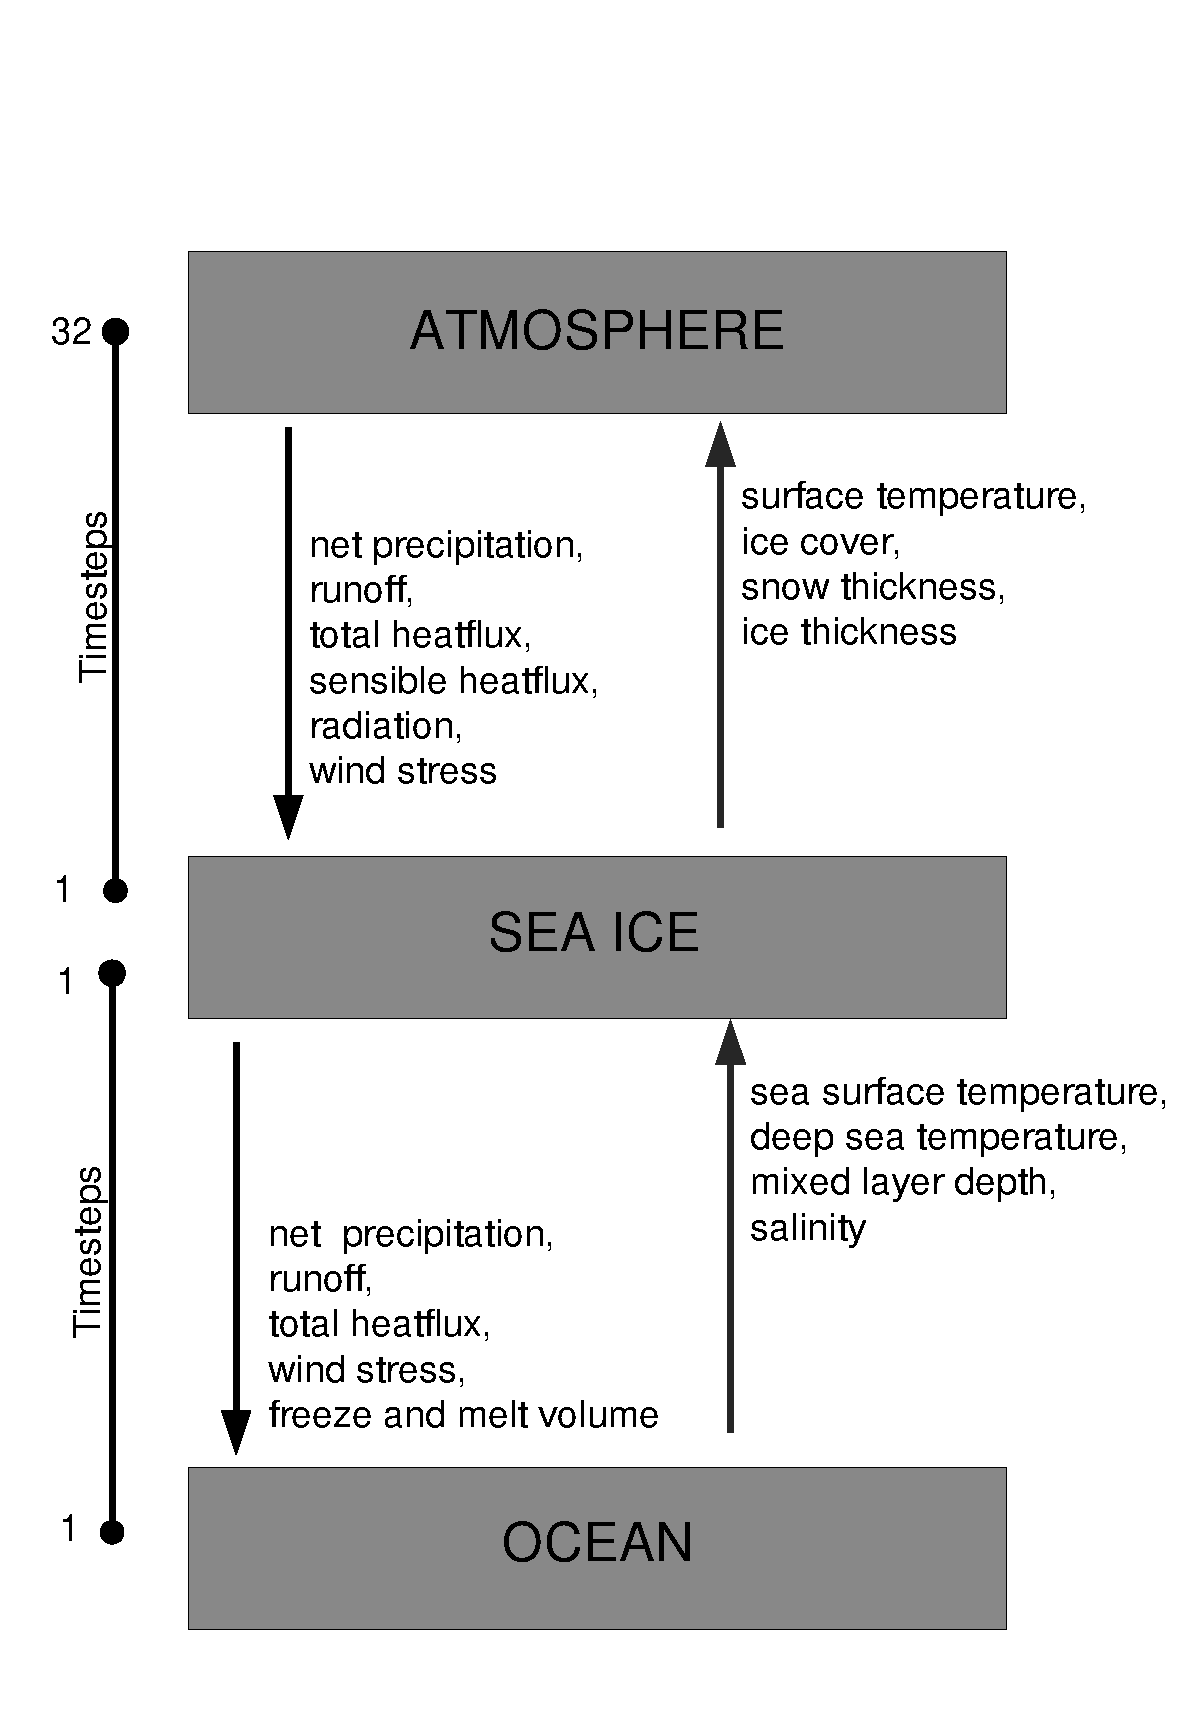
\includegraphics[width={14cm}]{Pics/modules_icemod_couple}
\caption[]{Schematic illustration of the model coupling.}
\label{couplefig}
\end{figure}

\begin{figure}[p]
\vspace{-2cm}
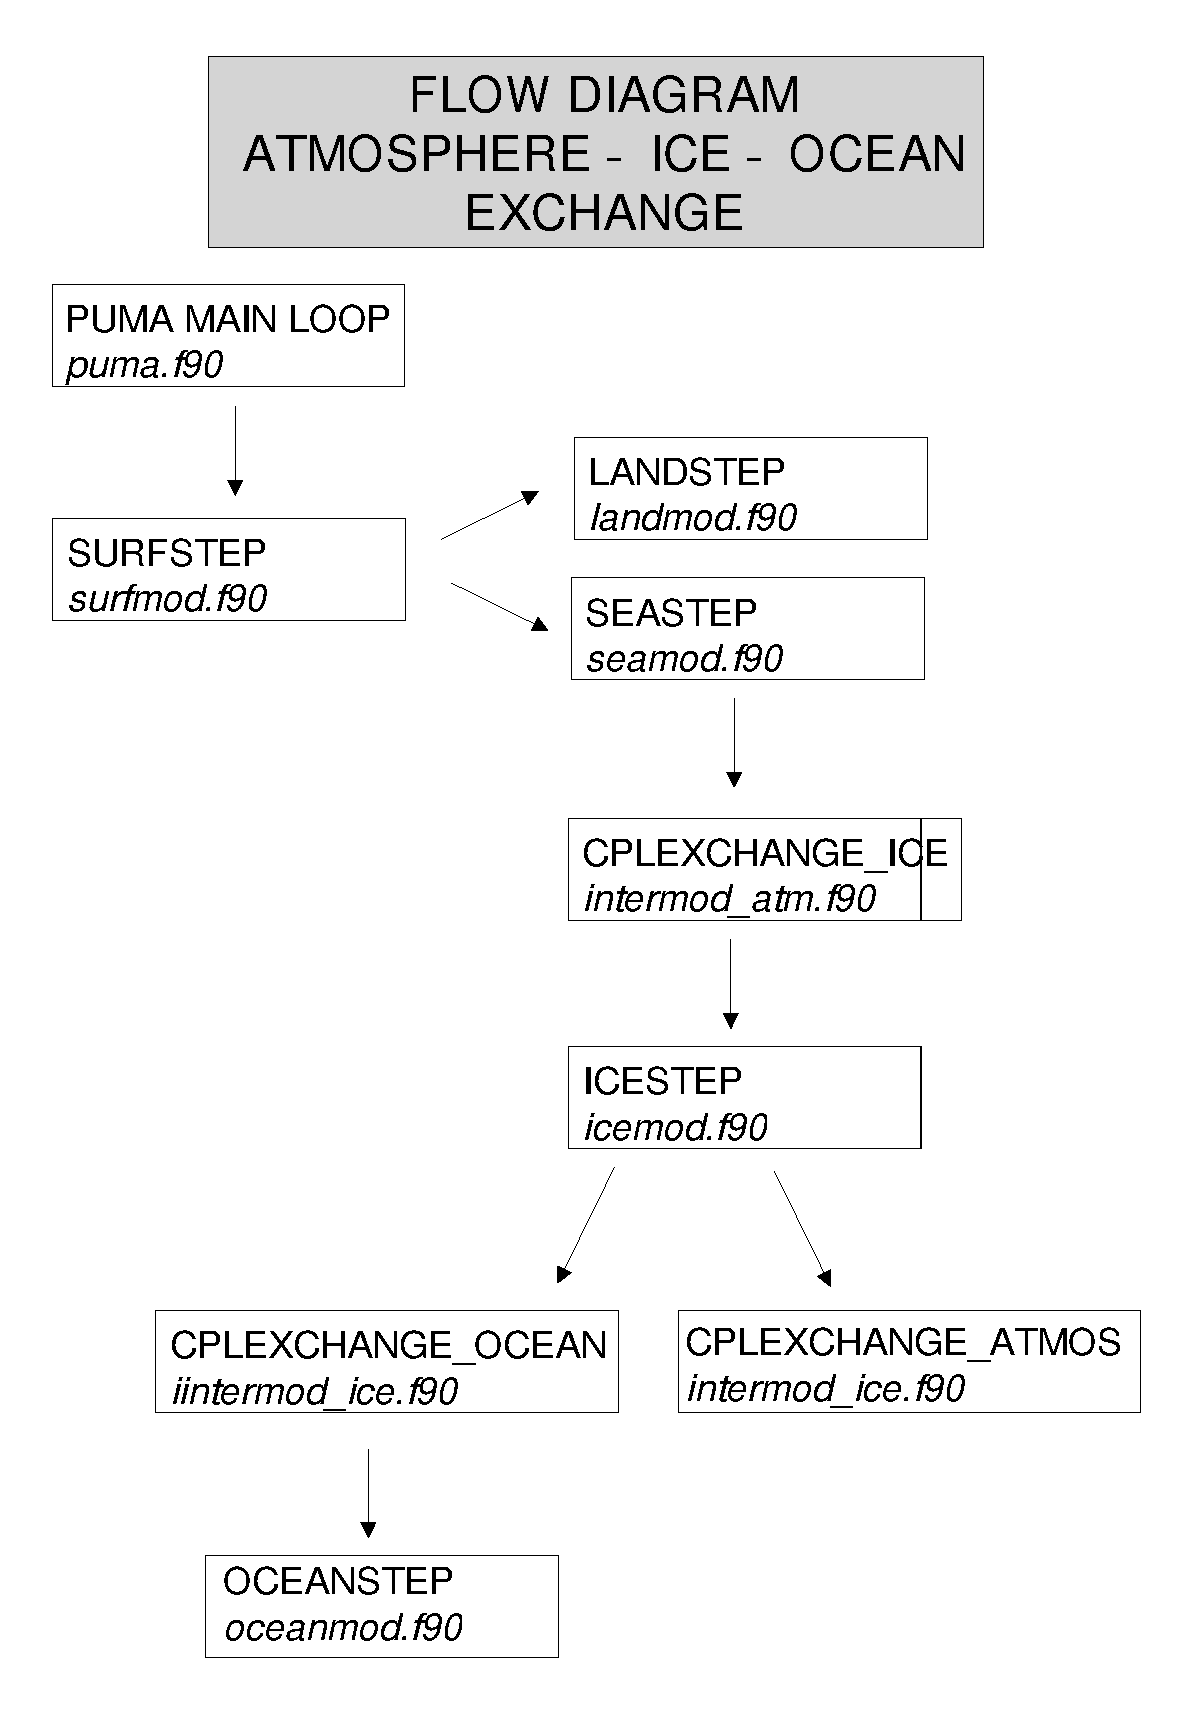
\includegraphics[width={14cm}]{Pics/modules_icemod_pumaflow}
\caption[]{Subroutine flow when no external coupler is used.}
\label{pumaflowfig}
\end{figure}


%----------------------------------------------------------------------------

\clearpage
\begin{center}
\begin{tabular}{|p{14cm}|}
\hline
\vspace{-5mm} \section{icemod.f90} \vspace{-5mm} \\
\hline
\vspace{1mm} {\bf General} The module {\module icemod.f90}
contains subroutines to compute sea ice cover and thickness.
The interface to the main PLASIM module is given by the subroutine
{\sub icestep}, which is called by {\sub cplexchange\verb#_#ice}
(defined in {\module intermod\verb#_#atm.f90}), which is called by
{\sub seastep} (defined in {\module seamod.f90}). \vspace{3mm} \\
\hline
\vspace{1mm} {\bf Input/Output} {\module icemod.f90} requires the file
{\file ice\verb#_#flxcor} if NFLXCORR is set to a negative value.
If NOUTPUT is set to 1, the output files {\file fort.75} containing
global fields of ice model data and the file {\file fort.76}
containing diagnostic ice data are produced (for details,
see the reference manual). Both output files are in service format.
The module is controlled by the namelist {\nam icepar} in the file
{\file ice\verb#_#namelist}. \vspace{1mm} \\
\begin{tabular}{p{3cm} p{2cm} p{6cm} p{2cm}}
Parameter  & Type    & Purpose 					& default \\
NDIAG	   & INTEGER & Diagnostic output every NDIAG time steps	& 160	  \\
NOUT	   & INTEGER & Model data output every NOUT time steps	& 32	  \\
NOUTPUT	   & INTEGER & Icemodel output (0=no,1=yes)		& 1	  \\
NFLXCORR   & INTEGER & Time constant for restoring $(>0)$, no flux correction $(=0)$, use fluxcorrection from file $(<0)$ & $360\,d$ \\
\end{tabular} \vspace{3mm} \\
\hline
\vspace{2mm} {\bf Structure} {\module icemod.f90} uses the module
{\modu icemod} which is not dependent on the module {\modu pumamod}.
Subroutine {\sub iceini} reads the namelist and, when required,
the flux correction from the file {\file ice\verb#_#flxcor}.
Subroutine {\sub icestep} calls {\sub cplexchange\verb#_#atmos}
(defined in {\module intermod\verb#_#ice}) to get the atmospheric
forcing fields. If the {\nam sea\verb#_#namelist} parameter NICE is
set to 1, the subroutine {\sub subice} is called, which calculates
ice cover and thickness. Otherwise, climatological data, interpolated
to the current time step by {\sub iceget} are used. If an ice cover
is present, the surface temperature is calculated in {\sub skintemp}.
Otherwise, the surface temperature is set to the sea surface temperature
calculated by the ocean model. Every NCPL\verb#_#ICE\verb#_#OCEAN
(defined in {\nam sea\verb#_#namelist}) time steps, the external
subroutine {\sub cplexchange\verb#_#ocean} (defined in
{\module intermod\verb#_#ice}) is called to pass the atmospheric
forcing to and retrieve oceanic data from the ocean module
{\module oceanmod.f90}. The oceanic data is used for ice calculations
in the next time step. \vspace{3mm} \\
\hline
\end{tabular}
\end{center} 

%--------------------------------------------------------------------------------

\clearpage
\begin{center}
\begin{tabular}{|p{14cm}|}
\hline
\vspace{-5mm} \section{oceanmod.f90} \vspace{-5mm} \\
\hline
\vspace{1mm} {\bf General} The module {\module oceanmod.f90} contains
a mixed layer ocean model, i.e. subroutines to compute sea surface
temperature and mixed layer depth. The interface to the main PLASIM
module is via the module {\module icemod.f90} given by the subroutine
{\sub oceanstep}, which is called by {\sub cplexchange\verb#_#ocean}
(defined in {\module intermod\verb#_#ice}).  \vspace{3mm} \\
\hline
\vspace{1mm} {\bf Input/Output} {\module oceanmod.f90} requires the file {\file ocean\verb#_#flxcor} if NFLXCORRSST or NFLXCORRMLD is set to a negative value. If NOUTPUT is set to 1, the output file {\file fort.31} containing global fields of ocean model data in service format is produced (for details, see the ice modul section of the reference guide). The module is controlled by the namelist {\nam oceanpar} in the file {\file ocean\verb#_#namelist}. \vspace{1mm} \\
\begin{tabular}{p{3cm} p{2cm} p{6cm} p{2cm}}
Parameter   & Type    & Purpose 			        & default \\
NDIAG	    & INTEGER & Diagnostic output every NDIAG time steps	& 480	  \\
NOUT	    & INTEGER & Model data output every NOUT time steps	& 32	  \\
NOUTPUT	    & INTEGER & Oceanmodel output (0=no,1=yes)		& 1	  \\
NFLXCORRMLD & INTEGER & Time constant for restoring mixed layer depth $(>0)$, no flux correction $(=0)$, use fluxcorrection from file $(<0)$ & $60\,d$ \\
NFLXCORRSST & INTEGER & Time constant for restoring sea surface temperature $(>0)$, no flux correction $(=0)$, use fluxcorrection from file $(<0)$ & $60\,d$ \\
\end{tabular} \vspace{3mm} \\
\hline
\vspace{2mm} {\bf Structure} {\module oceanmod.f90} uses the module
{\modu oceanmod} which is not dependent on the module {\modu pumamod}.
Subroutine {\sub oceanini} reads the namelist and, when required,
the flux corrections from the file {\file ocean\verb#_#flxcor}.
Subroutine {\sub oceanstep} calls {\sub mixocean}, which calculates
mixed layer depth and temperature. If an ice cover is present, mixed
layer depth is set to the climatological value and the sea surface
temperature is set to the freezing temperature. For details of the
mixed layer model, see the Planet Simulator Reference Manual.  \vspace{3mm} \\
\hline
\end{tabular}
\end{center} 

%------------------------------------------------------------------------




\chapter{Parallel Program Execution}
\section{Concept}

The {\bf Planet Simulator} is coded for parallel execution
on computers with multiple CPU's or networked machines.
The implementation uses MPI (Message Passage Interface),
that is available for nearly every operating system
{\url{http://www.mcs.anl.gov/mpi}}.

In order to avoid maintaining two sets of source code
for the parallel and the single CPU version, all
calls to the MPI routines are encapsulated into a module.
Users, that want to compile and execute the parallel
version use the module
{\bf mpimod.f90} and the commands {\bf mpif90}
for compiling and {\bf mpirun} for running.

If MPI is not implemented or the single CPU
version is sufficient, {\bf mpimod\_stub.f90}
is used instead of {\bf mpimod.f90}.
Also remove or comment the line:
\begin{verbatim}
!     use mpi
\end{verbatim}
and set the number of processors to 1:
\begin{verbatim}
      parameter(NPRO = 1)
\end{verbatim}




\section{Parallelization in Gridpoint Domain}

The data arrays in gridpoint domain are either 
three-dimensional e.g. gt(NLON, NLAT, NLEV) referring
to an array organized after longitudes, latitudes and levels,
or two-dimensional, e.g. gp(NLON, NLAT).
The code is organized such, that there are no dependencies
in latitudinal direction, while in gridpoint domain.
Such dependencies are resolved during the Legendre-Transformations.
So the the partitioning of the data is done in latitudes.
The program can use as many CPU's as latitudes with the extreme
of every CPU doing the computations for a single latitude.
There is the restriction however, that the number of latitudes
(NLAT) divided by the number of processors (NPRO), giving
the number of latitudes per process (NLPP) must have zero
remainder. E.g. A T31 resolution uses $NLAT=48$.
Possible values for NPRO are then 1, 2, 3, 4, 6, 8, 12, 16, 24, and 48.

All loops dealing with a latitudinal index look like:
\begin{verbatim}
      do jlat = 1 , NLPP
         ....
      enddo
\end{verbatim}

There are, however, many subroutines, with the most prominent
called {\bf calcgp}, that can fuse latitudinal and longitudinal
indices. In all these cases the dimension NHOR is used.
NHOR is defined as: $NHOR = NLON * NLPP$ in the 
pumamod - module. The typical gridpoint loop that looks like:

\begin{verbatim}
      do jlat = 1 , NLPP
         do jlon = 1 , NLON
            gp(jlon,jlat) = ...
         enddo
      enddo
\end{verbatim}

is then replaced by the faster executing loop:

\begin{verbatim}
      do jhor = 1 , NHOR
         gp(jhor) = ...
      enddo
\end{verbatim}

\section{Parallelization in Spectral Domain}

The number of coefficients in spectral domain (NRSP)
is divided by the number of processes (NPRO) giving
the number of coefficients per process (NSPP).
The number is rounded up to the next integer and the
last process may get some additional dummy elements,
if there is a remainder in the division operation.

All loops in spectral domain are organized like:

\begin{verbatim}
      do jsp = 1 , NSPP
         sp(jsp) = ...
      enddo
\end{verbatim}

\section{Synchronization points}

All processes must communicate and have therefore to
be synchronized at following events:

\begin{itemize}

\item Legendre-Transformation: 
This involves changing from latitudinal partitioning to
spectral partitioning and such some gather and scatter
operations.

\item Inverse Legendre-Transformation:
The partitioning changes from spectral to latitudinal
by using gather, broadcast, and scatter operations.

\item Input-Output:
All read and write operations must be done only by
the root process, who gathers and broadcasts or
scatters the information as desired.
Code that is to be executed by the root process exclusively is 
written like:

\begin{verbatim}
   if (mypid == NROOT) then
      ...
   endif
\end{verbatim}

NROOT is typically 0 in MPI implementations,
mypid (My process identification) is assigned by MPI.

\end{itemize}


\section{Source code}

It needs some discipline in order to maintain parallel code.
Here are the most important rules for changing or adding code
to the {\bf Planet Simulator}:

\begin{itemize}

\item Adding namelist parameters:
   All namelist parameters must be broadcasted after reading
   the namelist. (Subroutines mpbci, mpbcr, mpbcin, mpbcrn)

\item Adding scalar variables and arrays:
   Global variables must be defined in a module header
   and initialized. 

\item Initialization code:
   Initialization code, that contains dependencies on
   latitude or spectral modes must be done by the
   root process only and then scattered from there
   to all child processes.

\item Array dimensions and loop limits:
   Always use parameter constants (NHOR, NLAT, NLEV, etc.)
   as defined in
   pumamod.f90 for array dimensions
   and loop limits. 

\item Testing:
   After significant code changes the program should be tested 
   in single and in multi-CPU configuration. The results
   of a single CPU run is usually not exactly the same as the
   result of a multi-CPU run due to effects in
   rounding. But the results should show only small
   differences during the first timesteps.

\item Synchronization points:
   The code is optimzed for parallel execution and minimizes
   therefore communication overhead. The necessary communication
   code is grouped around the Legendre-transformations.
   If more scatter/gather operations or other communication
   routines are to be added, they should be placed
   just before or after the execution of the calls to the
   Legendre-Transformation. Any other place would degrade
   the overall performance in introducing additional
   process synchronization.

\end{itemize}




\chapter{Graphical User Interface}
\label{chap_GUI}
\section{Graphical user interface (GUI)}
\label{sec_GUI}

\begin{figure}
   \centering
   \includegraphics[width=8.5cm]{Pics/mostsnap}
   \caption[]{Screenshot of Model Starter (MoSt)}
   \label{mostsnap}
\end{figure}

The {\model} may be used in the traditional fashion,
with shell scripts, batch jobs, and network queuing 
systems. This is acceptable for long running simulations
on complex machines and number-crunchers, like vector-
computers, massive-parallel-computers and workstation clusters.
There is now, however, a much more convenient method by using
a graphical user interface (GUI) for model setup with parameter configurations
and for interaction between user and model.


The {\model} is configured and setup by the first
GUI module named MoSt (Model Starter, screenshot in \ref{mostsnap}). 
MoSt is the fastest way to get the
model running. It gives access to the most important parameters of
the model preset to the most frequently used values.
The model can be started with a mouse click on the button
labelled "Save \& Run" either with the standard paramater setting
or after editing some of the parameters in the MoSt window.
Some parameters, like horizontal and vertical resolution,
or the number of processors, require the building
(compile, link and load) of new executables. MoSt achieves
this by generating and executing build scripts,
that perform the necessary code changes and
create the required executable.
Other parameters define startup- and
boundary conditions or settings for parameterisations.
They can be edited in MoSt and, after a check for
correct range and consistency with other parameters,
are written to the model's namelist file.

Depending on all settings
MoSt generates a runscript for the simulation.
The user has the choice of leaving MoSt and
continue with the simulation under control of a GUI
right away, or to exit MoSt with the scripts prepared
to run. The second alternative is useful for users, who
want to modify the setup beyond the scope of MoSt
or want to run the Planet Simulator without GUI.

There's also a simple graphical editor for topograpy.
Check the box Orography and then use the mouse to mark
rectangular areas in the topography display.
Enter a value for rising (positive) or lowering the area
and press the button labelled {\bf Preprocess}.
The preprocessor will be built and executed, a new
topography will be computed and written to a start file.

Another editor is the mode editor for spherical harmonics.
Green modes are enabled, red modes are disabled.
This feature can be used to make runs with only certain
modes of spherical harmonics being active.
MB1, MB2, MB3 refer to the left, middle, and right mouse
button. You may toggle individual modes or whole lines
and columns. Currently this mode editor can only be used
for {\model} in the T21 resolution.

\begin{figure}
   \centering
   \includegraphics[width=8.5cm]{Pics/guisnap}
   \caption[]{Screenshot of Graphical User Interface (GUI)}
   \label{guisnap}
\end{figure}

The GUI for running the {\model}
(screenshot in \ref{guisnap})
has two main purposes. The first one is to display
model arrays in suitable representations.
Current implementations are:
\begin{itemize}
\item{Zonal mean cross sections}
\item{Horizontal global fields in cylinder projection}
\item{Horizontal global fields in polar projection}
\item{Time-longitude (Hovmoeller) diagrams}
\item{Amplitudes of coefficients of spherical harmonics}
\item{Time series}
\item{Numerical values}
\end{itemize}

In case of horizontal global grids pressing the MMB (Middle Mouse Button)
toggles between cylinder and polar projection. If the grid is
just one level from many of a three dimensional field like u or v,
the level shown can be decreased by the LMB or increased by the RMB.
For Hovmoeller and longitude height sections the LMB and RMB can
be used to select the latitude.

The second purpose is the interaction part of the GUI, which allows the user to change
selected model variables during the model run.
It is not necessary, though possible, to pause the
model while changing variables. Changes to model variables
are, of course, monitored in the outputfile and checked
by GUI for the appropriate range of values and
maximum possible change per timestep because, 
otherwise, a rapid parameter change or a choice of values beyond the normal
range may blow up the model.

All model variables, which are candidates for the display
or interactive changes, have a special code to communicate
with the Planet Simulator. The experienced modeller
can add new code for more variables using the existing
communication code as template. Thus all model fields
or even fields received via coupling with other models
can be put on the GUI display.

Both, MoSt and GUI are implemented using the Xlib (X11R5),
which is a library of routines for graphics and event communication.
As this library is part of every UNIX/Linux operating system
and base of all desktop environments, there is no need
to install additional software for running MoSt and GUI.
Another important  property of Xlib is the full network transparency.
The display of MoSt and GUI is not locked to the machine
running the programs or the model. In fact, the best
performance is obtained in running the Planet Simulator on
two or four CPUs of a remote server while displaying
the GUI on the user's workstation.
In summarizing, the MoSt and GUI programs automate many tedious tasks,
minimize the time to become familiar with the Planet Simulator,
and make debugging and parameter tuning much easier.
More kinds of presentations, coordinate projections
and interactivity are being developed.
A graphical preprocessor with editor for boundary
conditions and a graphical postprocessor are future expansions
to build an almost complete environment for modellers.

\section{GUI configuration}

On initialization the GUI reads its configuration from a file
{\bf GUI.cfg} which must be present in the current directory.
MoSt copies the file {\bf GUI.cfg} from the ../dat/ directory
to the run directory while building the {\model}.
After reading {\bf GUI.cfg} an attempt is made to read the file
{\bf GUI\_last\_used.cfg}. This file is always written at the end
of a GUI controlled simulation. So one may rearrange and position
GUI windows during a run and the new layout will be saved to the
file {\bf GUI\_last\_used.cfg}. In order to make this user
layout default for following runs, just copy this file like:
\begin{verbatim}
Most15/plasim/run$ cp ../dat/GUI.cfg ../dat/GUI.cfg.old
Most15/plasim/run$ cp GUI_last_used.cfg ../dat/GUI.cfg
\end{verbatim}
MoSt will then copy your new layout to the run directory at 
the next invocation.

The {\bf GUI.cfg} is a text file that may be also edited manually.
There is a section for each window (counting from 0 to 8) which
looks like:

\begin{verbatim}
[Window 00]                       <- window number (0..8)
Array:CSU                         <- array name
Plot:ISOCS                        <- picture type
Palette:U                         <- colour palette
Title:Zonal Wind [m/s]            <- window title
Geometry:  529  299    2    3     <- width height left top

[Window 01]
Array:SPAN
Plot:ISOSH
Palette:AMPLI
Title:Spherical Harmonics Ps
Geometry:  529  299  535    3

...

\end{verbatim}

Possible values for these items are:

\subsection{Array}
\begin{tabular}{|l|l|}
\hline
Name     & Description \\
\hline
CSU      & Cross Section U - Zonal mean zonal wind \\
CSV      & Cross Section V - Zonal mean meridional wind \\
CST      & Cross Section T - Zonal mean temperature \\
SPAN     & Spherical harmonics coefficients of surface pressure \\
GU       & Three dimensional grid of zonal wind \\
GV       & Three dimensional grid of meridional wind \\
GP       & Grid of surface pressure \\
DQVI     & Vertically integrated humidity \\
GUCOL    & sounding of eastward wind at a grid point \\
GVCOL    & sounding of northward wind a grid point \\
GTCOL    & sounding of temperature at a grid point \\
DQCOL    & sounding of humidity at a grid point \\
DQLCOL   & sounding of liquid water at a grid point \\
DCCCOL   & sounding of cloud cover at a grid point \\
SCALAR   & Selected scalars for timeseries and tables \\
\hline
\end{tabular}

\subsection{Plot}
\begin{tabular}{|l|l|}
\hline
Name     & Description \\
\hline
   ISOHOR & Isolines and colouring of horizontal grids \\
   ISOCS &  Isolines and colouring of cross sections \\
   ISOHOV & Colouring of Hovmoeller diagram \\
   ISOTS &  Timeseries \\
   ISOTAB & Tables \\
   ISOSH &  Coloured amplitudes \\
   ISOLON & Isolines and colouring of longitude height section \\
   ISOCOL & vertical Hovmoeller diagram for soundings \\
\hline
\end{tabular}

\subsection{Palette}
\begin{tabular}{|l|l|l|}
\hline
Name     & Range & Description  \\
\hline
   AUTO & automatic & rainbow colours \\
   U &    -10 .. 50 & rainbow colours \\
   V &    -10 .. 10 & rainbow colours \\
   T &    -50 .. 50 & blue - red \\
   P &    985 .. 1025 & blue - red \\ 
   Q &      0 .. 60 & rainbow colours \\
   DCC   &  0 ..100 & rainbow colours \\
   MARST & -90 .. 0 & blue -red \\
   AMPLI & 0 .. 12 & blue - green -red \\
   VEG   & 0 .. 100 & shades of green \\
\hline
\end{tabular}

\subsection{Title}
The title item may contain any text, but keep it short,
the length of the window's title bar is limited.
The words {\em Latitude} and {\em Level} have special
features in conjunction with threedimensional arrays,
where the user may scroll the level or latitude.
The GUI will insert the level number after the world 
{\em Level} or the latitude after the word {\em Latitude}.

\subsection{Geometry}
The four integers following the geometry item describe
the size and screen position of the window.
The first two parameters refer to width and height in 
screen pixel. These are the sizes of the inner window,
title bar, border and other decorations are not counted.
The third and fourth parameter set the coordinates of the
upper left corner of the window x and y, again without borders.
If the geometry item is not defined, the GUI will
initialize the window's geometry depending on the screen size.




\chapter{Postprocessor Pumaburner}
\label{Pumaburner}
\section{Introduction}

The {\bf Pumaburner} is a postprocessor for the {\bf Planet Simulator}
and the {\bf PUMA} model family.
It is the only interface between the {\it raw} model output data
and the diagnostics, graphics, and user software.

The output data of {\bf PUMA} is stored as
packed binary (16 bit) values using the model representation.
Prognostic variables such as temperature, divergence, vorticity,
pressure and humidity are stored as coefficients of spherical harmonics
on $\sigma$ levels. Variables like radiation,
precipitation, evaporation, clouds and other fields of the
parameterization package are stored on Gaussian grids.

The tasks of the {\bf Pumaburner} are:
\begin{itemize}
\item Unpack the {\it raw} data to full real representation.
\item Transform variables from the model's representation
      to a user selectable format, e.g. grids,
      zonal mean cross sections, and Fourier coefficients.
\item Calculate diagnostic variables, such as vertical velocity,
      geopotential height, wind components, etc.
\item Transfrom variables from $\sigma$ levels to user
      selectable pressure levels.
\item Compute monthly means and standard deviations.
\item Write selected data either in SERVICE or NetCDF format
      for further processing.
\end{itemize}

\section{Installation / Compilation}

The Pumaburner doesn't have to be installed, in most cases a compilation
of the source code and the storage of the executable in a "bin" directory
is sufficient. E.g.:

\begin{verbatim}
c++ -O2 -o burn6 burn6.cpp -lm -lnetcdf_c++ -lnetcdf
\end{verbatim}

The NetCDF library version 3 or higher must be installed on the computer,
otherwise the above command will fail with an error.
On some computer sites NetCDF might be installed, but the include or 
library search paths may lack the right configuration. In those cases either
ask your administrator to update the configuration or specify the
necessary locations on the compiler command using "-I" to specify the path
for "Include" files and "-L" for library files. Of course other C++ compilers,
like g++ for example may be used as well. If you're not the admin of your
system, put the executable burn6 into your \$HOME/bin directory.
This is normally part of your search path.

\section{Usage}

\begin{verbatim}
burn6 [options] InputFile OutputFile <namelist >printout
     option -h : help (this output)
     option -c : print available codes and names
     option -d : debug mode (verbose output)
     option -g : write GRADS control file for SERVICE data file
     option -n : NetCDF output (override namelist option)
     option -m : Mean=1 output (override namelist option)
     InputFile : Planet Simulator or PUMA data file
    OutputFile : SERVICE or NetCDF format file
      namelist : redirected <stdin>
      printout : redirected <stdout>
\end{verbatim}

\section{Namelist}

The namelist values control the selection, coordinate system
and output format of the postprocessed variables.
Names and values are not case sensitive.
Values can be assigned to the following names: \vspace{0.4cm}

\begin{tabular}{|l|c|l|l|l|}
\hline
Name   & Def. & Type & Description & Example \\
\hline
{\bf HTYPE    }& S & char & Horizontal type                 & HTYPE=G \\
{\bf VTYPE    }& S & char & Vertical type                   & VTYPE=P \\
{\bf MODLEV   }& 0 & int  & Model levels                    & MODLEV=2,3,4 \\
{\bf hPa      }& 0 & real & Pressure levels                 & hPa=500,1000 \\
{\bf LATS     }& 0 & int  & No. of latitudes for output grid  & LATS=40      \\
{\bf LONS     }& 0 & int  & No. of longitudes for output grid & LONS=80      \\
{\bf CODE     }& 0 & int  & ECMWF field code                & CODE=130,152 \\
{\bf NETCDF   }& 0 & int  & NetCDF output selector          & NETCDF=1 \\
{\bf CYCLICAL }& 0 & int  & Add data for longitude=360      & CYCLICAL=0 \\
{\bf MEAN     }& 1 & int  & Compute monthly means           & MEAN=0 \\
{\bf HHMM     }& 1 & int  & Time format in Service format   & HHMM=0 \\
{\bf HEAD7    }& 0 & int  & User parameter                  & HEAD7=0815 \\
{\bf MARS     }& 0 & int  & Use constants for planet Mars   & MARS=1 \\
{\bf MULTI    }& 0 & int  & Process multiple input files    & MULTI=12 \\
\hline
\end{tabular}

\section{HTYPE}

{\bf HTYPE} accepts the first character of the following string.
The following settings are equivalent: HTYPE = S, HTYPE=Spherical Harmonics
HTYPE = Something. Blanks and the equals sign are optional. \\
Possible Values are: \vspace{0.4cm}

\begin{tabular}{|l|l|l|}
\hline
   Setting   & Description          & Dimension for T21 resolution   \\
\hline
   HTYPE = S & Spherical Harmonics  & (506):(22 * 23 coefficients)   \\
   HTYPE = F & Fourier Coefficients & (32,42):(latitudes,wavenumber) \\
   HTYPE = Z & Zonal Means          & (32,levels):(latitudes,levels) \\
   HTYPE = G & Gaussian Grid        & (64,32):(longitudes,latitudes) \\
\hline
\end{tabular}

\section{VTYPE}

{\bf VTYPE} accepts the first character of the following string.
The following settings are equivalent: VTYPE = S, VTYPE=Sigma,
VTYPE = Super. Blanks and the equals sign are optional. \\
Possible Values are: \vspace{0.4cm}

\begin{tabular}{|l|l|l|}
\hline
   Setting   & Description          & Remark \\
\hline
   VTYPE = S & Sigma (model) levels & Some derived variables are not available \\
   VTYPE = P & Pressure levels      & Interpolation to pressure levels \\
\hline
\end{tabular}

\section{MODLEV}

{\bf MODLEV} is used in combination with {\bf VTYPE = S}.
If VTYPE is not set to ``Sigma'', the contents of MODLEV are ignored.
MODLEV is an integer array that can have as many values as there are
levels in the model output. The levels are numbered from the top of
the atmosphere to the bottom. The number of levels and the 
corresponding $\sigma$ values are listed in the Pumaburner printout.
The levels are ordered in the output file  according to the MODLEV values.
MODLEV=1,2,3,4,5 produces an output file of five model levels
sorted from top to bottom, while MODLEV=5,4,3,2,1 sorts them
from bottom to top.

\section{hPa}

{\bf hPa} is used in combination with {\bf VTYPE = P}.
If VTYPE is not set to ``Pressure'', the contents of hPa are ignored.
hPa is a real array that accepts pressure values with the
units hectoPascal or millibar. All output variables will be
interpolated to the selected pressure levels.
There is no extrapolation at the top of the atmosphere.
For pressure values, which are lower than that at the model's
top level, the top level value of the variable is taken.
The variables, temperature and geopotential height, are extrapolated
if the selected pressure is higher than the surface pressure.
All other variables are set to the value of the lowest mode level
for this case. The outputfile contains the levels in the same order
as they are set in hPa. For example: hpa = 100,300,500,700,850,900,1000.

\section{LATS and LONS}

        The Pumaburner defaults to the dimension of the model run.
        E.g. $Lats=32$ and $Lons=64$ for a T21 resolution.
        Note however, that this results in Gaussian grids with
        non equidistant latitudes.
        Selecting for Lats and Lons values, that are different from
        the internal resolution produces equidistant lat-lon grids.
        Lats sets the number of latitudes from north to south,
        with the North Pole at index 1 and the South Pole at index Lats.
        Delta Phi is therefore 180 degrees / (Lats - 1).
        Lons sets the number of gridpoints on every latitude circle.
        Delta Lambda is 360 / Lons.
        Index 1 is on the Greewich Meridian (0 degrees), while the last index
        denotes the point (360 degrees - Delta Lambda).
        Technical note:
           Variables that are stored as spherical harmonics
        (Temperature, vorticity, divergence, etc.) are calculated
        on the user grid by setting up the Legendre Transformation
        and the FFT accordingly. Variables, that are stored on
        Gaussian grids are interpolated with a bilinear interpolation.
        Note: Lats $>= 8$ and Lons $>= 16$ due to technical reasons.


\section{MEAN}

{\bf MEAN} can be used to compute monthly means and/or deviations.
The Pumaburner reads date and time information from the model file
and handles different lengths of months and output intervals correctly. 
\vspace{0.4cm}

\begin{tabular}{|l|p{12cm}|}
\hline
Setting & Description \\
\hline
        MEAN  =  0 & Do not average - all terms are processed. \\

        MEAN  =  1 & Compute and write monthly mean fields.
                     Not for spherical harmonics, Fourier coefficients, or
                     zonal means on sigma levels. \\

        MEAN  =  2 & Compute and write monthly deviations.
                     Not for spherical harmonics, Fourier coefficients, or
                     zonal means on sigma levels.
                     Deviations are not available for NetCDF output. \\

        MEAN  =  3 & A combination of MEAN=1 and MEAN=2.
                     Each mean field is followed by a deviation
                     field with an identical header record.
                     Not for spherical harmonics, Fourier coefficients, or
                     zonal means on sigma levels. 
		     Deviations are not available for NetCDF output. \\
\hline
\end{tabular}

\section{Format of output data}

The {\bf Pumaburner} supports two different output formats:

\begin{itemize}
\item {\bf NetCDF} (Network Common Data Format)
\item {\bf Service} Format for user readable data (see below).
\end{itemize}

For more detailed descriptions see for example:

{\url{http://www.nws.noaa.gov/om/ord/iob/NOAAPORT/resources/}}

\begin{tabular}{|l|p{10cm}|}
\hline
Setting & Description \\
\hline
   NetCDF = 1 & The output file is written in NetCDF format. \\
   NetCDF = 0 & The output file is written in Service format. \\
\hline
\end{tabular}

\section{SERVICE format}

     The SERVICE format uses the following structure:
     The whole file consists of pairs of
     header and data records.
     The header record is an integer array of 8 elements.

\begin{verbatim}
     head(1) = ECMWF field code
     head(2) = model level or pressure in [Pa]
     head(3) = date  [yymmdd]  (yymm00 for monthly means)
     head(4) = time  [hhmm]  or [hh] for HHMM=0
     head(5) = 1. dimension of data array
     head(6) = 2. dimension of data array
     head(7) = may be set with the parameter HEAD7
     head(8) = experiment number (extracted from filename)

     Example for reading the SERVICE format (NETCDF=0)

     INTEGER HEAD(8)
     REAL    FIELD(64,32)     ! dimensions for T21 grids
     READ (10,ERR=888,END=999) HEAD
     READ (10,ERR=888,END=999) FIELD
     ....
 888 STOP 'I/O ERR'
 999 STOP 'EOF'
     ....
\end{verbatim}

A new command line parameter "-g" was added for users of the GRADS
graphics software. Using -g in conjunction with SERVICE output
creates a GRADS control file describing the contents of the SERVICE
data file. GRADS can now be used to process the SERVICE data without
using converters or utilities (see chapter 7).


\section{HHMM}

\begin{tabular}{|l|p{12cm}|}
\hline
Setting & Description \\
\hline
  HHMM  =  0 & head(4) shows the time in hours (HH). \\
  HHMM  =  1 & head(4) shows the time in hours and minutes (HHMM). \\
\hline
\end{tabular}

\section{HEAD7}
The 7th element of the header is reserved for the user.
It may be used for experiment numbers, flags or anything else.
Setting HEAD7 to a number exports this number to every header record
in the output file (SERVICE format only).

\section{MARS}
This parameter is used for processing simulations of the Martian atmosphere.
Setting MARS=1 switches gravity, gas constant and planet radius
to the correct values for the planet Mars.

\section{MULTI}
The parameter MULTI can be used to process a series of input data during
 one run of the Pumaburner. Setting MULTI to a number (n)
tells the Pumaburner to process (n) input files.
The input files must follow one of these two rules:
\begin{itemize}
\item YYMM rule: The last four characters of the filename 
                 contain the date in the form YYMM.
\item .NNN rule: The last four characters of the filename
                 consist of a dot followed by a three digit sequence number.
\end{itemize}

\begin{verbatim}
Examples:

Namelist contains MULTI=3
Command: pumaburn <namelist >printout run.005 out
Result: Pumaburn processes the files <run.005> <run.006> <run.007>

Namelist contains MULTI=4
Command: pumaburn <namelist >printout exp0211 out
Result: Pumaburn processes the files <exp0211> <exp0212> <exp0301> <exp0302>
\end{verbatim}

\section{Namelist example}
\begin{verbatim}
       VTYPE  = Pressure
       HTYPE  = Grid
       CODE   = 130,131,132
       hPa    = 200,500,700,850,1000
       MEAN   = 0
       NETCDF = 0
\end{verbatim}

    This namelist will write Temperature(130), u(131) and v(132)
    to the pressure levels 200hPa, 500hPa, 700hPa, 850hPa and 1000hPa.
    The output interval is the same as that found on the model data,
    e.g. every 12 or every 6 hours (MEAN=0). The output format
    is the SERVICE format.

\section{Troubleshooting}
If the Pumaburner reports an error or does not produce 
the expected results, try the following:

\begin{itemize}

\item Check your namelist, especially for invalid codes, types and levels.

\item Run the Pumaburner in debug-mode by using the option -d.
For example:
\begin{verbatim}
pumaburn <namelist >printout -d data.in data.out
\end{verbatim}

This will print out details such as the parameters and the memory allocation used
during the run. This additional information may help to diagnose the problem.

\item Not all combinations of HTYPE, VTYPE, and CODE are valid.
Try using HTYPE=Grid and VTYPE=Pressure before switching to more
exotic parameter combinations.

\end{itemize}



\chapter{Graphics}
\section{Grads}
In this section, visualisation using the graphics package GrADS is
described. A useful Internet site for reference and installation
instructions is
\begin{quote}
\verb#<http://grads.iges.org/grads/grads.html>#.
\end{quote}
Latest versions of \verb#GrADS# can handle data in \verb#NETCDF#
format (via the command
\verb#sdfopen#), \verb#GRIB#, \verb#HDF-SDS#, and in its native binary
format. The native format can
conveniently be derived from \verb#SERVICE# format.
In the following it is assumed that the \verb/PUMA/ output has been
 converted to \verb#SERVICE# format with the \verb#pumaburner# and the
resulting
file is called \verb/puma.srv/. Monthly mean data is either obtained
directly from the \verb#pumaburner# (\verb#namelist# parameter
\verb#MEAN=1#, see section \ref{Pumaburner}) or via a
\verb/PINGO/ command:
\begin{quote}
\verb/srv monmeans puma.srv puma_m.srv/
\end{quote}
\noindent Information on the \verb/PINGO/ package can be
found in DKRZ report 11 at
\begin{quote}
 \verb#<http://www.mad.zmaw.de/Pingo/repdl.html>#.
\end{quote}
The \verb#SERVICE# file has to be converted to
\verb#GrADS#'s native format by the command:
\begin{quote}
\verb#srv2gra puma_m.srv#
\end{quote}
\noindent which results in the files \verb/puma_m.gra/ and
\verb/puma_m.ctl/. The first file contains the data, the latter one
information on the grid, time steps, and variable names. The program
\verb#srv2gra# is one of the postprocessing tools available at
\begin{quote}
\verb#<http://puma.dkrz.de/puma/download/map/>#.
\end{quote}
If you chose to compile it yourself, please read the comments in the
first few lines of the program text.
Sometimes the
\verb/srv2gra/ tool has difficulties to calculate an appropriate time
increment from the date headers of the data records, so you should
check this. In this example the file \verb/puma_m.ctl/ should look like this:
\begin{verbatim}
DSET ^puma_m.gra
UNDEF 9e+09
XDEF     64 LINEAR   0.0000   5.6250
OPTIONS YREV
YDEF     32 LEVELS 
  -85.7606  -80.2688  -74.7445  -69.2130  -63.6786  -58.1430  -52.6065  -47.0696
  -41.5325  -35.9951  -30.4576  -24.9199  -19.3822  -13.8445   -8.3067   -2.7689
    2.7689    8.3067   13.8445   19.3822   24.9199   30.4576   35.9951   41.5325
   47.0696   52.6065   58.1430   63.6786   69.2130   74.7445   80.2688   85.7606
ZDEF  1 LINEAR 1 1
TDEF 12 LINEAR 00:00Z01jan0001        1mo
VARS  3
c139     0 99    139     0     0
c151     0 99    151     0     0
c175     0 99    175     0     0
ENDVARS
\end{verbatim}
Here, the line starting with \verb/TDEF/ ends with \verb/1mo/, since
we are handling monthly mean data. When the \verb/PUMA/ output is used
without averaging, this should correspond to the output interval given
by the \verb#nafter# variable used in the \verb#namelist# of your \verb#PUMA#
run (see section \ref{Namelist}). The number of variables
depends on how the pumaburner was
called. In this example, only 3 variables were processed, i.e.\ the
surface temperature (\verb/c139/), the sea level pressure
(\verb/c151/) and the albedo (\verb/c175/; refer to appendix
\ref{Pumacodes} for a list of codes).
\\
The GrADS program is started by typing \verb/grads/ in a terminal window. Then, data is visualised either by typing commands line-by-line, or, preferably, by using scripts. The following script, called \verb/tglob.gs/, displays the monthly mean surface temperature:
\begin{verbatim}
# tglob.gs
function pass(m)
'reinit'
'open puma_m'
'enable print print.mf'
'set t 'm
'c'
'set gxout shaded'
'd (c139-273.16)'
'cbar.gs'
'set gxout contour'
'd (c139-273.16)'
'draw title Surface Temperature (deg C) month 'm
'print'
'disable print'
'!gxps -i print.mf -o tglob'm'.ps'
\end{verbatim}
The variable \verb/m/ at the beginning of the script defines the month which should be displayed. It is passed from the terminal with the script call. Note that in this line, no quotation marks are present, since only \verb/GrADS/ specific commands are framed by quotation marks. Script commands, like variable definitions, if-clauses etc. are used without quotation marks. The script is executed by typing its name without the ending and the number of the month to be shown. For example, \verb/tglob 7/ displays the monthly mean surface temperature in July. The resulting output file is called \verb/tglob7.ps/. 
\par
\vspace{3mm}
The following script \verb/thh/ displays the time dependent surface temperature of Hamburg. Here, two variables are passed to \verb/GrADS/, the first and last day to plot (note that here, the file \verb/puma.gra/ is opened, which contains data on a daily basis). The call \verb/thh 91 180/ displays the surface temperature of Hamburg for the spring season from April 1st to June 30th.

\begin{verbatim}
# thh.gs
function pass(d1 d2)
'reinit'
'open puma'
'enable print print.mf'
'set lat 53'
'set lon 10'
'set t 'd1' 'd2
'c'
'd (c139-273.16)'
'draw title Surface Temperature (deg C) in Hamburg'
'print'
'disable print'
'!gxps -i print.mf -o thh.ps'
\end{verbatim}

\vspace{3mm}
It is possible to have more than one figure in a plot, which is illustrated in the following script. It plots seasonal means of the sea level pressure. The data file is prepared like this:

\begin{verbatim}
srv selcode,151 puma.srv slp.srv
srv seasmean slp.srv slp_sm.srv
srv2gra slp_sm.srv
\end{verbatim}

The commands \verb/set vpage/ sets virtual pages inside the graphic window. The full window is 11 inch wide and 8.5 inch high, so \verb/set vpage 0 5.5 4.25 8.5/ defines the upper left corner. If \verb/setlevs=1/ is specified, the pressure levels as given are used. Otherwise, \verb/GrADS/ defines contour levels depending on the data set.

\begin{verbatim}
# slp_sm.gs
setlevs=1
'reinit'
'open slp_sm'
'enable print print.mf'
'c'
'set vpage 0 5.5 4.25 8.5'
'set gxout contour'
if (setlevs=1)
'set clevs 990 995 1000 1005 1010 1015 1020'
endif
'set ccols 1'
'set grads off'
'set t 1'
'd c151/100'
'draw title SLP [hPa] yr 'ny' DJF'
'set vpage 5.5 11 4.25 8.5'
'set gxout contour'
if (setlevs=1)
'set clevs 990 995 1000 1005 1010 1015 1020'
endif
'set ccols 1'
'set grads off'
'set t 2'
'd c151/100'
'draw title yr 'ny' MAM'
'set vpage 0 5.5 0 4.25'
'set gxout contour'
if (setlevs=1)
'set clevs 990 995 1000 1005 1010 1015 1020'
endif
'set ccols 1'
'set grads off'
'set t 3'
'd c151/100'
'draw title yr 'ny' JJA'
'set vpage 5.5 11 0 4.25'
'set gxout contour'
if (setlevs=1)
'set clevs 990 995 1000 1005 1010 1015 1020'
endif
'set ccols 1'
'set grads off'
'set t 4'
'd c151/100'
'draw title yr 'ny' SON'
'print'
'disable print'
'!gxps -c -i print.mf -o slp_sm.ps'
\end{verbatim}

\section{Vis5D}
\begin{quote}
{\it ``Vis5D is a system for interactive visualization of large 5-D
gridded data sets such as those produced by numerical weather
models. One can make isosurfaces, contour line slices, colored slices,
volume renderings, etc of data in a 3-D grid, then rotate and animate
the images in real time. There's also a feature for wind trajectory
tracing, a way to make text annotations for publications, support for
interactive data analysis, etc.''}
\par
\end{quote}
\begin{flushright}
from the Vis5D home page,\\
{\url{http://www.ssec.wisc.edu/~billh/vis5d.html}}
\end{flushright}
\par
\noindent This powerful visualisation tool together with its documentation is
available through the above home page. Vis5D uses its own data format
which makes it necessary to transform your data. Depending on their
format
% (see also section \ref{Filestructure}
 and the flowchart on
{\url{http://puma.dkrz.de/puma/download/map/}} you have the following
choices: If

\begin{itemize}
\item{{\it your data is raw \verb#PUMA# output,}\\
	you need to process it with the \verb#pumaburner#
	postprocessor (see section \ref{Pumaburner}) in order to
	transform it to either
	\verb#NETCDF#} (option \verb#-n# or namelist parameter
	\verb#NETCDF=1#) or \verb#GRIB# (option \verb#-g# or namelist
	parameter \verb#GRIB=1#) and proceed from there.
\item{{\it your data is in \verb#SERVICE# format,}\\
	you need to convert it to either \verb#GRIB#, for
	instance with the \verb#PINGO#s:
\begin{quote}
 \verb#grb copy2 data.srv data_with_grib_metainfo.grb output.grb#,
\end{quote}	
	or \verb#NETCDF#,
	using the program \verb#puma2cdf#, which is available with the
	\verb#PUMA# postprocessing tools. Despite of its name this
	program cannot process raw \verb#PUMA# output but takes
	\verb#SERVICE# format as input. It can as well be called as
	\verb#srv2cdf# which changes its behaviour: oddities of model
	output such as the existence of February, $30^{th}$ are
	then no longer removed.	Once the format is changed proceed from there.}
\item{{\it your data is in \verb#NETCDF# format,}\\
	it can easily transformed to \verb#Vis5D#'s native format by
	means of the program \verb#cdf2v2d#, which is available with
 	the \verb#PUMA# postprocessing tools.}
\item{{\it your data is in \verb#GRIB# format,\\}
	you can find a transformation tool named \verb#Grib2V5d# at\\
	\verb#<http://grib2v5d.sourceforge.net># which offers various
	practical features.}
\end{itemize}
\noindent Once the conversion to \verb#Vis5D#'s native format is
	achieved please follow the instructions from the \verb#Vis5D#
	documentation or, if \verb#Vis5D# is already installed on your
	system, try finding your own way by typing:
\begin{quote}
\verb#vis5d my_data.v5d#
\end{quote}




\chapter{Column Mode and Soundings}
 \section{Setup}

The column mode of the the Planet Simulator is an integral part 
of the full Planet Simulator and not a stand alone model. 
The advantage of this approach is that all options and modules 
available in the full model are automatically included in
the column mode and that no extra maintenance is necessary. 

Technically this is realized by switching off horizontal 
advection and diffusion which leaves us with an independent
column for each grid point. The inclusion of additional options
for boundary conditions allows for runs with synchronized columns.   

Running the Model at the lowest resolution (T1) with  $8$ 
synchronized columns is efficient enough to
run very fast column integrations. Using a standard setup
with $10$ atmospheric layers and a mixed layer ocean one 
can simulate more than $33500$ years per day on a single 
processor PC (3.3 GHZ CPU).

To make full use of the computer power one can setup an ensemble of 
columns by specifying boundary conditions for every grid point 
separately.

\subsection{Basic switches for column setup}

We introduce the macro switch {\bf COLUMN} in the namelist {\it inp}
which is part of the namelist $\mathrm{ \bf puma{\_}namelist}$.
By setting {\bf  COLUMN = 1} a default column mode is initialized by
setting {\bf YMODE = "Column"}, {\bf KICK = 0}, {\bf NADV = 0}
and {\bf NHORDIF = 0}. One can customize the column setup by keeping
the default value {\bf  COLUMN = 0} and by setting the other switches
individually. For more details see the table {\it inp}
in appendix \ref{Namelist}.  

\subsection{Boundary Conditions and forcing}

For the T1 truncation the following lower boundary conditions are specified
by external fields: The land sea mask 
($\mathrm{N002\_surf\_0172.sra}$), 
the surface geopotential ($\mathrm{N002\_surf\_0129.sra}$)
and the surface temperature ($\mathrm{N002\_surf\_0169.sra}$).
The other fields are set by default within the model. Some can be
set by namelist parameters (see description of standard model).

The surface fluxes of heat and moisture in the 
column mode can be influenced by the switch {\bf ZUMIN} 
in the namelist {\it fluxpar} which sets the surface wind 
speed entering the bulk exchange scheme. The default value 
is set to 1 m/s.

Keeping the standard settings the columns will be forced by the solar
forcing corresponding to the grid point where the column is located.
For the T1 truncation this mean that the columns are located approximately
at gaussian latitudes $\pm 35.26^\circ$. The solar forcing corresponds
to the default of the full model. A daily mean insolation is
used with an annual cycle. The solar forcing is also influenced
by the climatological ozon distribution which by default also has
an annual cycle.


\section{Graphical User Interface (GUI)}

To visualize the time evolution of the column model a vertical Hovmoeller 
plot has been added to the GUI (picture type: ISOCOL).
The sounding device can be also used to visualize the vertical profiles at 
an arbitrary grid point of the gaussian grid in the full model. 
By clicking the window the sounding goes from grid point to grid point 
in meridional direction. The longitude can be selected by the switch 
{\bf sellon}, which is a parameter of the {\bf inp} namelist in 
$\mathrm{\bf puma\_namelist}$.  
Using the template $\mathrm{GUI\_sounding.cfg}$ in folder 
{\bf plasim/dat} the GUI is configured for soundings. 
In this case {\bf sellon} can be modified in the control window. 
For more details see chapter \ref{chap_GUI}. 


% \chapter{Diagnostics}
% \section{Fluxes}

% \chapter{Reference Simulation}

\begin{appendix}
\chapter{List of Constants and Symbols}
\label{locs}
\begin{tabular*}{\textwidth}{|l@{\extracolsep\fill}lll|}
\hline
\vspace{-3mm} & & & \\
Symbol         & Definition                       & Value   & Unit \\
\hline 
\vspace{-3mm} & & & \\
$a$       & earth radius                          & $\rm 6371\e{3}$ & $\rm
m$ \\
$A$       & $=D+\vec{V} \cdot \nabla \ln p_s $         &         & $\rm -$ \\
${\cal A}$      &  absorptivity/emissivity                                           &                     & $\rm -$ \\
${\cal A}_S$  & surface emissivity                                              &         &$\rm -$ \\
$B(T)$            & Planck function                    &    &$\rm Wm^{-2}$ \\
$cc$      & cloud cover                 &    & $\rm -$\\
$C_{char}$     & Charnock constant                     & 0.018   & $\rm -$ \\
$C_h$          & transfer coefficient for heat         &         & $\rm -$ \\
$C_m$          & drag coefficient for momentum         &         & $\rm -$ \\
$c_p$          & specific heat of moist air at constant pressure      &         & $\rm J\,
kg^{-1}\, K^{-1}$ \\  
$c_{pd}$  & specific heat of dry air at constant pressure   & 1005.46      & $\rm J\,
kg^{-1}\, K^{-1}$ \\
$c_{pv}$  & specific heat of water vapor at constant pressure    & 1869.46      & $\rm J\,
kg^{-1}\, K^{-1}$ \\
$c_{p_i}$      & specific heat of sea ice              & 2070         & $\rm W\,
s\, kg^{-1}\, K^{-1}$ \\
$c_{p_s}$      & specific heat of snow            & 2090         & $\rm W\,
s\, kg^{-1}\, K^{-1}$ \\
$c_{p_w}$      & specific heat of sea water            & 4180         & $\rm W\,
s\, kg^{-1}\, K^{-1}$ \\
$c_w$          & coefficient for the deep ocean heat flux   & 4       & $\rm W\,
m^{-2}\, K^{-1}$ \\
$C_w$          & wetness factor                   &         & $\rm -$ \\

$D$       & scaled divergence                          &         & $\rm -$ \\

$E$       & evaporation                      &         & $\rm m\,
s^{-1}$ \\
$E_0$          & extrateristical solar flux density         &         & $\rm W\,
m^{-2}$ \\

$f$       & Coriolis parameter $=:2\Omega\sin\varphi$  &         & $\rm
s^{-1}$ \\
$F_p$          & tendency of the first moment$=:\frac{d R_{1}}{d t}$  &    &
$\rm K\, m^2\, s^{-1}$ \\
$F_q$          & tendency of the zeroth moment$=:\frac{d R_{0}}{d t}$ &    &
$\rm K\, m\, s^{-1}$ \\
$F_q$          & surface moisture flux            &         & $\rm kg\,
m^{-2}\, s^{-1}$ \\
$F_T$          & surface sensible heat flux            &         & $\rm W\,
m^{-2}$ \\
$F_u$          & surface zonal wind stress             &         & $\rm Pa$
\\
$F_v$          & surface meridional wind stress        &         & $\rm Pa$
\\
$F^{LW}$  & long wave radiation flux density      &    &$\rm  W m^{-2}$ \\
$F^{SW}$  & short wave radiation flux density     &    &$\rm  W m^{-2}$ \\
$g$       & gravitational acceleration            & 9.81         & $\rm
m^{-2}$ \\

$h_{mix}$      & mixed layer depth                     &         & $\rm m$ \\
$h_{mix_c}$    & climatological mixed layer depth           &         & $\rm m$ \\
$H_q$          & effective mixed layer depth $=:\frac{R_{0}}{T_{mix}-T_{ref}}$ &
& $\rm m$ \\
$H_p$          & reduced center of gravity $=:\frac{R_{1}}{R_0}$ &         &
$\rm m$ \\ 

\hline
\end{tabular*}
\newpage

\begin{tabular*}{\textwidth}{|l@{\extracolsep\fill}lll|}
\hline
\vspace{-3mm} & & & \\
Symbol         & Definition                       & Value   & Unit \\
\hline 
\vspace{-3mm} & & & \\

$J_q$          & vertical turbulent moisture flux           &         & $\rm kg\, m^{-2}\,
s^{-1}$ \\
$J_T$          & vertical turbulent temperature flux        &         & $\rm K\,
m^{-2}\, s^{-1}$ \\
$J_u$          & vertical turbulent flux of zonal momentum  &         & $\rm Pa$
\\
$J_v$          & vertical turbulent flux of meridional momentum &          & $\rm Pa$
\\

$k$       & von Karman constant                   & 0.4          & $\rm -$ \\
$K_h$          & exchange coefficient for heat         &         & $\rm -$ \\
$K_m$          & exchange coefficient for momentum          &         &$\rm -$ \\
$L$       & latent heat                      &         & $\rm J\, kg^{-1}$\\

$L_f$          & latent heat of fusion = $L_s - L_v$        & $\rm 3.28\e{5}$   &
$\rm J\, kg^{-1}$ \\
$l_h$          & mixing length for heat                &         & $\rm m$ \\
$l_m$          & mixing length for momentum            &         &
$\rm m$ \\
$L_s$          & latent heat of sublimation            & $\rm 2.8345\e{6}$ & $\rm J\,
kg^{-1}$ \\
$L_v$          & latent heat of vapourization               & $\rm 2.5008\e{6}$
     & $\rm J\, kg^{-1}$ \\
$P_c$     & convective precipitation    &    &$\rm  m s^{-1}$ \\
$P_l$     & large scale precipitation   &    &$\rm  m s^{-1}$ \\
$P^m_n(\mu)$   & associated Legendre function of the first kind &          & $\rm -$ \\
$p$       & pressure  \hspace*{\fill}             &         & $\rm Pa$ \\
$p_S$          & surface pressure                 &         & $\rm Pa$
\\
$p_s$          & scaled surface pressure               &         & $\rm -$ \\

$q$       & specific humidity                     &         & $\rm kg\,
kg^{-1}$ \\
$Q$       & total heat flux through sea ice       &         & $\rm W\, m^{-2}$
\\
$\tilde{Q}$    & flux correction heat flux through sea ice  &         & $\rm W\, m^{-2}$
\\
$Q_a$          & total atmospheric heat flux                &         & $\rm W\,
m^{-2}$ \\
$Q_c$          & conductive heat flux through sea ice       &         & $\rm W\,
m^{-2}$ \\
$Q_f$          & heat flux available for freezing sea ice   &         & $\rm W\, m^{-2}$
\\
$Q_g$     & heat flux into the soil     &    & $\rm W m^{-2}$ \\
$Q_m$     & snow melt heat flux    &    & $\rm W m^{-2}$ \\
$Q_o$          & oceanic heat flux                     &         & $\rm W\, m^{-2}$
\\
$q_S$          & surface specific humidity             &         & $\rm kg\,
kg^{-1}$ \\
$q_{sat}$      & saturation specific humidity               &         & $\rm kg\,
kg^{-1}$ \\
${\cal R}$     & refexivity/albedo      &    &$\rm -$ \\
${\cal R}_S$   & surface albedo    &    & $\rm -$ \\
$R_d$          & gas constant for dry air              & 287.05  & $\rm J\,
kg^{-1}\, K^{-1}$ \\
$R_l$          & surface long wave radiation           &         & $\rm W\,
m^{-2}$ \\
$R_s$          & surface short wave radiation               &         & $\rm W\,
m^{-2}$ \\
$R_v$          & gas constant for water vapor               & 461.51  &
$\rm J\, kg^{-1}\, K^{-1}$ \\
$R_{0}$   & zeroth moment of the temperature distribution   &         & $\rm K\,
m$ \\
$R_{1}$   & first moment of the temperature distribution    &         & $\rm K\,
m^2$ \\
$Ri$           & Richardson number                     &         & $\rm -$ \\ 
$S_w$          & salinity of sea water                 & 34.7    
     & $\rm psu$ \\

\hline
\end{tabular*}
\newpage

\begin{tabular*}{\textwidth}{|l@{\extracolsep\fill}lll|}
\hline
\vspace{-3mm} & & & \\
Symbol         & Definition                       & Value   & Unit \\
\hline 
\vspace{-3mm} & & & \\

$t$       & time                             &         & $\rm s$ \\
$t$       & scaled time step                      &         & $\rm -$ \\
${\cal T}$     & transmissivity    &    &$\rm  -$ \\
$T$       & temperature                      &         & $\rm K$
\\
$T'$           & temperature anomaly $=:T-T_0$              &         & $\rm -$ \\
$T_d$          & deep ocean temperature (at 400m)      &         & $\rm K$
\\
$T_i$          & sea ice surface temperature           &         & $\rm K$ \\
$T_f$          & freezing temperature                  & 271.25  & $\rm K$
\\
$T_s$          & surface temperature                   &         & $\rm K$
\\
$T_{sea}$ & sea surface temperature     &    & $\rm K$ \\
$T_{melt}$     & melting point                    & 273.16  & $\rm K$ \\
$T_{mix}$      & mixed layer temperature               &         & $\rm K$ \\
$T_{mix_c}$    & climatological mixed layer temperature     &         & $\rm K$
\\
$T_{ref}$      & asymptotic reference temperature           &         & $\rm K$ \\
$T_w$          & oceanic temperature profile                &         &
$\rm K$ \\
$T_0$          & reference temperature profile         &  250.0  & $\rm K$
\\

$U$       & scaled zonal wind $=:u\cdot\cos\varphi$    &         & $\rm -$ \\
$u$       & zonal wind                       &         & $\rm m\, s^{-1}$
\\
$u_*$          & friction velocity                          &         & $\rm m\, s^{-1}$ \\

$V$       & scaled meridional wind $=:v\cdot\cos\varphi$    &         & $\rm -$ \\
$v$       & meridional wind                  &         & $\rm m\, s^{-1}$
\\
$\vec{v}$      & horizontal wind vector                &         & $\rm m\, s^{-1}$
\\
$W_L$     & cloud liquid water path     &    & $\rm g m^2$ \\
$W_{snow}$ & mass of snow water    &    & $\rm kg $\\
$W_{soil}$     & soil water             &    & $\rm  m $\\
$z$       & height                      &    & $\rm m$ \\
$z_0$          & roughness length            &    & $\rm m$ \\
$\Delta t $    & time increment              &    & $\rm s$ \\
 $\Delta z $   & height increment            &    &$\rm  m$ \\
$\alpha$  & thermal expansion coefficient $\frac{1}{\rho} \frac{d\rho}{dT}$ & $\rm
2.41\e{-4}$ & $\rm K^{-1}$ \\
$\beta$   & back scattering coefficient &         &$\rm - $\\
$\beta_d$      & diffusivity factor          & 1.66    &$\rm - $ \\
$\zeta$   & scaled vorticity                      &         & $\rm -$ \\
$\theta$  & potential temperature            &         & $\rm K$ \\
$\kappa$  & $R_d/C_{pd}$                               &         & $\rm -$ \\
$\bar{\kappa}$      & mean heat conductivity in ice and snow     &         & $\rm W\,
m^{-1}\, K^{-1}$ \\
$\kappa_i$     & heat conductivity in ice              &  2.03   & $\rm W\, m^{-1}\,
K^{-1}$ \\
$\kappa_s$     & heat conductivity in snow             &  0.31   & $\rm W\,
m^{-1}\, K^{-1}$ \\

$\lambda_h$    & asymptotic mixing length for heat     &    &$\rm m $\\
$\lambda_m$    & asymptotic mixing length for momentum      &    &$\rm m $\\

$\lambda$      & longitude                                  &         & $\rm -$ \\

$\mu$          & $\sin\varphi$                              &         & $\rm -$ \\
$\mu_0$   & cosine of the solar zenith angle           &         & $\rm -$ \\ 

$\rho$         & density of air                   &         & $\rm kg\,
m^{-3}$ \\
$\rho_i$  & density of sea ice                    & 920          & $\rm kg\, m^{-3}$
\\
$\rho_s$  & density of snow                       & 330          & $\rm kg\, m^{-3}$
\\
$\rho_w$  & density of sea water                  & 1030         & $\rm kg\,
m^{-3}$ \\
$\rho_o$  & density of fresh water                & 1000    & $\rm kg\, m^{-3}$
\\

\hline
\end{tabular*}
\newpage

\begin{tabular*}{\textwidth}{|l@{\extracolsep\fill}lll|}
\hline
\vspace{-3mm} & & & \\
Symbol         & Definition                       & Value   & Unit \\
\hline 
\vspace{-3mm} & & & \\
$\sigma$  & normalized pressure coordinate $=: p/p_s$       &         & $\rm -$ \\
$\dot{\sigma}$  & vertical velocity in $\sigma$ system           &         & $\rm -$ \\
$\sigma_{SB}$ & Stefan-Bolzmann constant & $ 5.67 \e{-8}$ &$\rm W m^{-2}K^{-4}$ \\
$\tau_N$  & cloud optical depth    &    &$\rm  -$\\
$\tau_{F}$     & time scale for RF                     &         & $\rm -$ \\
$\tau_{R}$     & time scale for NC                     &         & $\rm -$ \\
$\tau_{T}$     & time scale for temperature flux correction      &         & $\rm s$ \\
$\tau_{h}$     & time scale for depth flux correction            &         & $\rm s$ \\

$\phi$         & geopotential height $:=g\cdot{z}$          &         & $\rm m^2\,
s^{-2}$ \\
$\phi$         & scaled geopotential height            &         & $\rm -$ \\
$\varphi$      & latitude                                   &         & $\rm -$ \\

$\chi$    & scaled velocity potential                  &         & $\rm -$ \\

$\psi$         & scaled streamfunction                      &         & $\rm -$ \\
$\Omega$  & angular velocity of the earth              & $\rm 7.292\e{-5}$ & $\rm
s^{-1}$ \\
$\tilde{\omega_0}$ & single scattering albedo     &    &$\rm- $\\

\hline
\end{tabular*}


\chapter{Planet Simulator Codes for Variables}
\label{Pumacodes}
\begin{table}[h]
Codes available from PUMA-burner \\

\begin{tabular}[t]{|l|l|l|l|l|} \hline
\multicolumn{1}{|c|}{Code} &
\multicolumn{1}{c|}{Levels}&
\multicolumn{1}{c|}{Type} &
\multicolumn{1}{c|}{Variable} &
\multicolumn{1}{c|}{Unit} \\ \hline \hline

129 & 1    & s  & surface geopotential             & m$^{2}$/s$^{2}$ \\ \hline
130 & NLEV & s  & temperature                      & K               \\ \hline
131 & NLEV & c  & u-velocity                       & m/s             \\ \hline
132 & NLEV & c  & v-velocity                       & m/s             \\ \hline
135 & NLEV & c  & vertical velocity                & Pa/s            \\ \hline
138 & NLEV & s  & vorticity                        & 1/s             \\ \hline
148 & NLEV & c  & horizontal streamfunction        & m$^{2}$/s       \\ \hline
149 & NLEV & c  & velocity potential               & m$^{2}$/s       \\ \hline
151 & 1    & c  & mean sea level pressure          & Pa              \\ \hline
152 & 1    & s  & ln(surface pressure)             &                 \\ \hline
154 & NLEV & s  & restoration temperature          & K               \\ \hline
155 & NLEV & s  & divergence                       & 1/s             \\ \hline
156 & NLEV & c  & geopotential height              & gpm             \\ \hline
\end{tabular}

\vspace*{0.5cm}

s: PUMA spectral field \\
c: computed by PUMA-burner \\

\end{table}

\chapter{Namelists}
\label{Namelist}
\section{File puma\_namelist}
\subsection{Namelist INP}
\begin{tabular}{|l|c|l|l|}                                  
\hline                                                        
{\bf Name      }&Def.&Type & Description \\               
\hline                                                        
{\bf column    }&   0 & int & 1: initialize PLASIM for column runs \\
{\bf kick      }&  1 & int & 0: no noise initialization ($p_s$ = const.) \\         
{\bf           }&     &     & 1: random white noise                \\
{\bf           }&     &     & 2: Equator symmetric random white noise  \\
{\bf           }&     &     & 3: mode (1,2) no random initialization  \\
{\bf mars      }&   0 & int & 1: initialize PLASIM for planet Mars \\
{\bf mpstep    }&  45 & int & minutes per step (lenghth of timestep) \\
{\bf nadv      }&   1 & int & 1: switches horizontal advection on \\
{\bf ncoeff    }&   0 & int & spectral coefficients to print in {\bf wrspam}\\
{\bf ndel(NLEV)}&all 2& int & order of hyperdiffusion for each level (2*h)\\
{\bf ndiag     }&  12 & int & output interval for diagnostics [timesteps] \\   
{\bf ndiagcf   }&   0 & int & 1: turn on cloud forcing diagnostic \\
{\bf ndiaggp   }&   0 & int & 1: process franks gp-diagnostic arrays \\
{\bf ndiaggp2d }&   0 & int & number of additional 2-d gp-diagnostic arrays \\
{\bf ndiaggp3d }&   0 & int & number of additional 3-d gp-diagnostic arrays  \\
{\bf ndiagsp   }&   0 & int & 1: process franks sp-diagnostic arrays \\
{\bf ndiagsp2d }&   0 & int & number of additional 2-d sp-diagnostic arrays \\
{\bf ndiagsp3d }&   0 & int & number of additional 3-d sp-diagnostic arrays \\
{\bf ndl(NLEV) }&all 0& int & 1: activate spectral printouts for this level \\
{\bf neqsig    }&   1 & int & 1: use equidistant sigma levels \\
{\bf nflux     }&   1 & int & 1: switches vertical diffusion on \\
{\bf ngui      }&   0 & int & 1: run with active GUI \\
{\bf nhdiff    }&  15 & int & critical wavenumber for horizontal diffusion \\
{\bf nhordif   }&   1 & int & 1: switches horizontal diffusion on \\
{\bf nkits     }&   3 & int & number of short initial timesteps \\       
{\bf noutput   }&   1 & int & enables (1) or disables (0) output file \\
{\bf npackgp   }&   1 & int & 1: pack gridpoint fields on output \\
{\bf npacksp   }&   1 & int & 1: pack spectral fields on output \\
{\bf nperpetual}&   0 & int & radiation day for perpetual integration \\
{\bf nprhor    }&   0 & int & 1: grid point for print out (only for checks!) \\
{\bf nprint    }&   0 & int & 1: comprehensive print out (only for checks!) \\
{\bf nrad      }&   1 & int & 1: switches radiation on  \\
{\bf ntime     }&   0 & int & 1: turn on time use diagnostics \\
{\bf nwpd      }&   1 & int & number of writes per day (to puma\_output) \\
\hline
\end{tabular}

\newpage

Namelist INP continued \vspace{3mm} \\
\begin{tabular}{|l|c|l|l|}                                  
\hline                                                        
{\bf Name      }&Def.&Type & Description \\               
\hline                                                        
{\bf n\_days\_per\_month} & 30 & int & length of month for simple calendar \\
{\bf n\_days\_per\_year} & 360 & int & length of year for simple calendar or 365 \\
{\bf n\_run\_days} & -1 & int & Simulation time (days to run) \\
{\bf n\_run\_months} & 0 & int & Simulation time (months to run) \\
{\bf n\_run\_years} & 1 & int & Simulation time (years to run) \\
{\bf n\_start\_month} & 1 & int & Starting month \\
{\bf n\_start\_year} & 1 & int & Starting year \\
{\bf psurf     }&101100.0&real& global mean surface pressure [Pa] \\
{\bf restim(NLEV)}&all 15.0 & real  & restoration timescale for each level \\ 
{\bf sigh(NLEV)} & all 0.0 & real & user definable sigmah array \\
{\bf sellon}    & 0.0 & real & longitude of soundings in the GUI \\
{\bf t0(NLEV)  }&all 250.0&real& reference $T_R$-temperature profile \\ 
{\bf tfrc(NLEV)}& 0,0,0,.. ,1  & int & Rayleigh friction timescale $\tau_F$ in days \\
{\bf tdissd    }& 0.2 & real  & diffusion time scale for divergence [days] \\
{\bf tdissq    }& 5.6 & real  & diffusion time scale for specific humidity [days] \\
{\bf tdisst    }& 5.6 & real  & diffusion time scale for temperature [days] \\
{\bf tdissz    }& 1.1 & real  & diffusion time scale for vorticity [days] \\
{\bf time0  }& 0.0 & real  & start time (for performance estimates) \\
\hline                                                        
\end{tabular}


\subsection{Namelist PLANET}
\begin{tabular}{|l|c|l|l|}                                  
\hline                                                        
{\bf Name      }&Def.&Type & Description \\               
\hline                                                        
{\bf akap         } & 0.286 & real & kappa \\
{\bf alr          } & 0.0065 & real & lapse rate \\
{\bf eccen        } & 0.0  & real & eccentricity for fixed orbits \\
{\bf ga           } & 9.81 & real & gravity \\
{\bf gascon       } & 287.0 & real & gas constant \\
{\bf mvelp        } & 0.0  & real & longitude of vernal equinox for fixed orbits (deg) \\
{\bf nfixorb      } & 0   & int & 1: fix the planetary orbit \\
{\bf obliq        } & 0.0  & real & obliquity for fixed orbits (deg) \\
{\bf plarad       } & 6371000.0 & real & planetary radius \\
{\bf pnu          } & 0.1 & real & time filter \\
{\bf ra1          } & 610.78 & real & parameter in Magnus-Teten formula \\
{\bf ra2          } & 17.269 & real & parameter in Magnus-Teten formula \\
{\bf ra4          } & 35.86 & real & parameter in Magnus-Teten formula \\
{\bf solar\_day   } & 86400.0 & real & length of solar day \\
{\bf siderial\_day} & 86164.0 & real & length of siderial day \\
{\bf ww           } & 7.29e-5 & real & $ 2 \pi / siderial day $ \\
{\bf yplanet      } & "Earth" & char & name of planet \\
\hline                                                        
\end{tabular}


\subsection{Namelist MISCPAR}
\begin{tabular}{|l|c|l|l|}                                  
\hline                                                        
Name   & Def. & Type & Description \\               
\hline                                                        
{\bf nfixer} & 1 & int & 1: correct negative moisture \\
{\bf nudge } & 0 & int & 1: temperature relaxation in the uppermost level \\
{\bf tnudge} & 10.0 & real & Time scale [d] of the temperature relaxation \\
\hline                                                        
\end{tabular}


\subsection{Namelist FLUXPAR}
\begin{tabular}{|l|c|l|l|}                                  
\hline                                                        
Name   & Def. & Type & Description \\               
\hline                                                        
{\bf nevap  }& 1 & int & 1: turn on surface evaporation \\  
{\bf nshfl  }& 1 & int & 1: turn on surface sensible heat flux \\
{\bf nstress }& 1 & int & 1: turn on surface wind stress \\
{\bf nvdiff  }& 1 & int & 1: turn on vertical diffusion \\
{\bf vdiff\_lamm  }& 160.0 & real & tuning parameter for vert. diff. \\
{\bf vdiff\_b  }& 5.0 & real & tuning parameter for vert. diff. \\
{\bf vdiff\_c }& 5.0 & real & tuning parameter for vert. diff. \\
{\bf vdiff\_d  }& 5.0 & real & tuning parameter for vert. diff. \\
{\bf zumin }& 1.0 & real & minimum surface wind speed (m/s) \\
\hline                                                        
\end{tabular}

  
\subsection{Namelist RADPAR}
\begin{tabular}{|l|c|l|l|}                                  
\hline                                                        
Name   & Def. & Type & Description \\               
\hline                                                        
{\bf acl2(3) } & 0.05,0.1,0.2 & real & cloud absorptivities spectral range 2 \\
{\bf acllwr  } & 0.1 & real & mass absorption coefficient for clouds (lwr) \\
{\bf clgray  } & -1.0 & real & cloud grayness \\
{\bf co2     } & 360.0 & real & co2 concentration (ppmv) \\
{\bf dawn    } & 0.0 & real & zenith angle threshhold for night \\
{\bf gsol0   } & 1365.0 & real & solar constant (w/m2) \\
{\bf iyrbp   } & -50 & int & Year before present (1950 AD); default = 2000 AD \\
{\bf ndcycle } & 0 & int & switch for daily cycle 1=on/0=off \\
{\bf nlwr    } & 1 & int & switch for long wave radiation (dbug) 1=on/0=off \\
{\bf no3     } & 1 & int & switch for ozon 1=on/0=off \\
{\bf nrscat  } & 1 & int & switch for rayleigh scattering (dbug) 1=on/0=off \\
{\bf nsol    } & 1 & int & switch for solar insolation (dbug) 1=on/0=off \\
{\bf nswr    } & 1 & int & switch for short wave radiation (dbug) 1=on/0=off \\
{\bf nswrcl  } & 1 & int & switch for computed or prescribed cloud props. 1=com/0=pres \\
{\bf rcl1(3) } & 0.15,0.3,0.6 & real & cloud albedos spectral range 1 \\
{\bf rcl2(3) } & 0.15,0.3,0.6 & real & cloud albedos spectral range 2 \\
{\bf th2oc   } & 0.04 & real & absorption coefficient for h2o continuum \\
{\bf tpofmt  } & 1.0 & real & tuning of point of mean (lwr) transmissivity in layer \\
{\bf tswr1   } & 0.04 & real & tuning of cloud albedo range1 \\
{\bf tswr2   } & 0.048 & real & tuning of cloud back scattering c. range2 \\
{\bf tswr3   } & 0.004 & real & tuning of cloud s. scattering alb. range2 \\
\hline                                                        
\end{tabular}


\subsection{Namelist RAINPAR}
\begin{tabular}{|l|c|l|l|}                                  
\hline                                                        
Name   & Def. & Type & Description \\               
\hline                                                        
{\bf clwcrit1   } & -0.1 & real & 1st critical vertical velocity for clouds \\
{\bf clwcrit2   } &  0.0 & real & 2nd critical vertical velocity for clouds \\
{\bf kbetta     } &  1   & int  & switch for betta in kuo (1/0=yes/no) \\
{\bf ncsurf     } &  1   & int  & conv. starts from surface (1/0=yes/no) \\
{\bf ndca       } &  1   & int  & dry convective adjustment (1/0=yes/no) \\
{\bf nmoment    } &  0   & int  & momentum mixing (1/0=yes/no) \\
{\bf nshallow   } &  0   & int  & switch for shallow convection (1/0=yes/no) \\
{\bf nprc       } &  1   & int  & large convective precip (1/0=yes/no) \\
{\bf nprl       } &  1   & int  & switch for large scale precip (1/0=yes/no) \\
{\bf rcrit(NLEV)} &      & real & critical relative hum. for non conv. clouds \\
\hline                                                        
\end{tabular}

  
\subsection{Namelist SURFPAR}
\begin{tabular}{|l|c|l|l|}                                  
\hline                                                        
Name   & Def. & Type & Description \\               
\hline                                                        
{\bf noromax  }& model resolution (NTRU) & int & resolution of orography \\
{\bf nsurf  }& not active & int & debug switch \\  
{\bf oroscale  }& 1.0 & real & scaling factor for orography \\
\hline                                                        
\end{tabular}


\section{File land\_namelist}
\subsection{Namelist LANDPAR}
\begin{tabular}{|l|c|l|l|}                                  
\hline                                                        
Name   & Def. & Type & Description \\               
\hline                                                        
{\bf  albgmax  } & 0.8   & real & max. albedo for glaciers \\
{\bf  albgmin  } & 0.6   & real & min. albedo for glaciers \\
{\bf  albland  } & 0.2   & real & albedo for land \\
{\bf  albsmax  } & 0.8   & real & max. albedo for snow \\
{\bf  albsmaxf } & 0.4   & real & max. albedo for snow (with forest) \\
{\bf  albsmin  } & 0.4   & real & min. albedo for snow \\
{\bf  albsminf } & 0.3   & real & min. albedo for snow (with forest) \\
{\bf  co2conv  } & 14.0  & real & co2 conversion factor \\
{\bf  drhsfull } & 0.4   & real & threshold above which drhs=1 [frac. of wsmax] \\
{\bf  drhsland } & 0.25  & real & wetness factor land \\
{\bf  dsmax    } & 5.00  & real & maximum snow depth (m-h20; -1 = no limit) \\
{\bf  dsoilz(NLSOIL)} &       & real & soil layer thickness \\
{\bf  dwatcini}  & 0.0   & real & soil water content (m) for manual 
                                  initialization   \\
                 &       &      &      (nwatcini=1) \\
{\bf  dz0land  } & 2.0   & real & roughness length land \\
{\bf  dzglac   } & -1.   & real & threshold of orography to be glacier (-1=none) \\
{\bf  dztop    } & 0.20  & real & thickness of the uppermost soil layer (m) \\
{\bf  forgrow  } & 1.0   & real & growth factor initialization \\
{\bf  gs       } & 1.0   & real & stomatal conductance initialization \\
{\bf  nbiome   } & 0     &  int & switch for vegetation model (1/0 : prog./clim) \\
{\bf  ncveg    } & 1     &  int & compute new dcveg (0=keep initial state) \\
{\bf  newsurf  } & 0     &  int & (dtcl,dwcl) 1: update from file, 2:reset  \\
{\bf  nlandt   } & 1     &  int & switch for land model (1/0 : prog./clim) \\
{\bf  nlandw   } & 1     &  int & switch for soil model (1/0 : prog./clim) \\
{\bf  nwatcini } & 0     &  int & switch for manual soil water setting (1/0 : on/off) \\
{\bf  rinisoil } &  0.0  & real & soil carbon initialization  \\
{\bf  riniveg  } &  0.0  & real & biomass carbon initialization \\
{\bf  rlaigrow } & 0.5   & real & above ground growth factor initialization \\
{\bf  rlue     } &  8.0E-10 & real & \\
{\bf  rnbiocats} &  0.0     & real & \\
{\bf  tau\_soil } & 42.0  & real & [years] - in landini scaled to seconds \\
{\bf  tau\_veg  } & 10.0  & real & [years] - in landini scaled to seconds \\
{\bf  wsmax    } & WSMAX\_EARTH & real & max field capacity of soil water (m) \\
{\bf  z0\_max   } & 2.0  &  real & maximum roughness length for vegetation \\
\hline                                                        
\end{tabular}


\section{File sea\_namelist}
\subsection{Namelist SEAPAR}
\begin{tabular}{|l|c|l|l|}                                  
\hline                                                        
Name   & Def. & Type & Description \\               
\hline                                                        
{\bf ncpl\_atmos\_ice  }& 32 & int & atmosphere ice coupling time steps \\
{\bf albsea  }& 0.069 & real & albedo for open water \\
{\bf albice  }& 0.7 & real & max. albedo for sea ice \\
{\bf dz0sea  }& $1.5\cdot 10^{-5}$ & real & roughness length sea [m]\\
{\bf dz0ice  }& $1.0\cdot 10^{-3}$ & real & roughness length ice [m]\\
{\bf drhssea  }& 1.0 & real & wetness factor sea \\
{\bf drhsice  }& 1.0 & real & wetness factor ice \\
\hline                                                        
\end{tabular}


\section{File ocean\_namelist}
\subsection{Namelist OCEANPAR}
\begin{tabular}{|l|c|l|l|}                                  
\hline                                                        
Name   & Def. & Type & Description \\               
\hline                                                        
{\bf dlayer(NLEV\_OCE)} & 50.0 & real & layer depth (m) \\
{\bf ndiag} & 480 & int & diagnostics each ndiag timestep \\
{\bf newsurf}& 0 & int & 1: read surface data after restart \\
{\bf nfluko}&  0 & int & switch for flux correction \\
{\bf nocean  }& 1 & int & ocean model (1) or climatology (0) \\  
{\bf nperpetual\_ocean}& 0 & int & perpetual climate conditions (day) \\
{\bf nprhor}& 0 & int & gridpoint for debug printout \\
{\bf nprint}& 0 & int & switch for debug printout \\
{\bf taunc}& 0.0 & real & time scale for newtonian cooling \\
{\bf vdiffk}& 1.0e-4 & real & vertikal diffusion coeff. [m**2/s] \\
\hline                                                        
\end{tabular}


\section{File ice\_namelist}
\subsection{Namelist ICEPAR}
\begin{tabular}{|l|c|l|l|}                                  
\hline                                                        
Name   & Def. & Type & Description \\               
\hline                                                        
{\bf newsurf}& 0 & int & 1: read surface data after restart \\
{\bf nfluko}&  0 & int & switch for flux correction \\
{\bf nice  }& 1 & int & sea ice model (1) or climatology (0) \\
{\bf nout  }& 32 & int & model data output every {\bf nout} time steps \\
{\bf nperpetual\_ice}& 0 & int & perpetual climate conditions (day) \\
{\bf nprhor}& 0 & int & gridpoint for debug printout \\
{\bf nprint}& 0 & int & switch for debug printout \\
{\bf nsnow}& 1 & int & allow snow on ice yes/no (1/0) \\
{\bf ntskin}& 1 & int & compute skin temperature (0=clim. \\
{\bf ncpl\_ice\_ocean  }& 1 & int & ice ocean coupling time steps \\
{\bf taunc}& 0.0 & real & time scale for newtonian cooling \\
{\bf xmind}& 0.1 & real & minimal ice thickness (m) \\
\hline                                                        
\end{tabular}



\end{appendix}

\end{document}

